%% LyX 2.3.7 created this file.  For more info, see http://www.lyx.org/.
%% Do not edit unless you really know what you are doing.
\documentclass[english,t,presentation]{beamer}
\usepackage{mathpazo}
\usepackage[T1]{fontenc}
\usepackage[utf8]{inputenc}
\setcounter{secnumdepth}{3}
\setcounter{tocdepth}{3}
\usepackage{babel}
\usepackage{float}
\usepackage{textcomp}
\usepackage{url}
\usepackage{bm}
\usepackage{multirow}
\usepackage{amssymb}
\usepackage{graphicx}
\ifx\hypersetup\undefined
  \AtBeginDocument{%
    \hypersetup{unicode=true,
 bookmarks=false,
 breaklinks=false,pdfborder={0 0 1},backref=section,colorlinks=false}
  }
\else
  \hypersetup{unicode=true,
 bookmarks=false,
 breaklinks=false,pdfborder={0 0 1},backref=section,colorlinks=false}
\fi

\makeatletter

%%%%%%%%%%%%%%%%%%%%%%%%%%%%%% LyX specific LaTeX commands.
%% Because html converters don't know tabularnewline
\providecommand{\tabularnewline}{\\}

%%%%%%%%%%%%%%%%%%%%%%%%%%%%%% Textclass specific LaTeX commands.
% this default might be overridden by plain title style
\newcommand\makebeamertitle{\frame{\maketitle}}%
% (ERT) argument for the TOC
\AtBeginDocument{%
  \let\origtableofcontents=\tableofcontents
  \def\tableofcontents{\@ifnextchar[{\origtableofcontents}{\gobbletableofcontents}}
  \def\gobbletableofcontents#1{\origtableofcontents}
}

%%%%%%%%%%%%%%%%%%%%%%%%%%%%%% User specified LaTeX commands.
% Created 2020-05-22 Fri 01:41
% Intended LaTeX compiler: pdflatex

\usepackage{grffile}
\usepackage{longtable}
\usepackage{wrapfig}
\usepackage{rotating}
\usepackage[normalem]{ulem}
\usepackage{textcomp}
\usepackage{capt-of}
%\usepackage[english]{babel}
\date{\tiny\printdayoff\today}
\usefonttheme{professionalfonts}
\usefonttheme{serif}
\usepackage{aecompl}
\usepackage{multimedia}
\usepackage{ifthen}
\usepackage{ulem}
\usepackage{bm}
\usepackage[]{url}
\usepackage{beamerthemesplit}
\usepackage{beamerthemeshadow}
\usepackage{booktabs}
\usepackage{subfigure}
\usepackage{textcomp}
\usepackage{textpos}
%\usepackage{unicode-math}
\usetheme{Antibes}

\usecolortheme{crane}
\author{Albert S. Kim\textsuperscript{1}, Kwang-Jin Lee\textsuperscript{2}, Moo-Seok Lee\textsuperscript{2}, Hyeon-Ju Kim\textsuperscript{3}, and Jung-Hyun Moon\textsuperscript{4}  \\ \vspace{.25cm} \\  \tiny   \textsuperscript{1}Civil and Environmental Engineering, University of Hawaii at Manoa, 2540 Dole Street, Holmes 383, Honolulu, Hawai'i, 96822 \\ \vspace{.1cm} \\  \textsuperscript{2}Business Division 2, Kolon Industries, Inc., KOLON One\&only tower, Magokdong-ro 110, Gangseo-gu, Seoul 07793, Republic of Korea \\ \vspace{.1cm} \\  \textsuperscript{3}Offshore Plant and Marine Energy Research Division, Korea Research Institute of Ships and Ocean Engineering, 32 Yuseong-Daero, 1312 Beon-Gil, Daejeon 305-343, Republic of Korea \\ \vspace{.1cm} \\  \textsuperscript{4}Seawater Energy Plant Research Center, Korea Research Institute of Ships \& Ocean Engineering (KRISO), 32 Yuseong-Daero 1312 Beon-Gil, Yuseong-Gu, Daejeon, KOREA \vspace{-.75cm}}
\date{May 21, 2020, NAMS2020 online}
\title{Hydrodynamic load exerted on}
\subtitle{a moving bundle of hollow fibers  using constraint dissipative hydrodynamics: Hydro-Rattle simulation}
\definecolor{UBCblue}{rgb}{0.04706, 0.13725, 0.26667} % UBC Blue (primary)
\definecolor{UBCgrey}{rgb}{0.3686, 0.5255, 0.6235} % UBC Grey (secondary)
\definecolor{ao(english)}{rgb}{0.0, 0.5, 0.0}
\definecolor{darkblue}{rgb}{0.097656, 0.097656, 0.43750}
\definecolor{darkgreen}{rgb}{0.0, 0.2, 0.13}
\definecolor{dartmouthgreen}{rgb}{0.05, 0.5, 0.06}
\definecolor{hawaiigray}{rgb}{0.88281, 0.88281, 0.88281}   % Hex=#E2E2E2
\definecolor{hawaiigreen}{rgb}{0.0078125, 0.27734, 0.19141}   % Hex=#024731
\setbeamercolor*{title}{bg=green}
\setbeamercolor{structure}{fg=dartmouthgreen}
\setbeamercolor{frametitle}{fg=yellow!20}
\setbeamercolor{frametitle}{fg=brown,bg=white}
\setbeamercolor{frametitle}{fg=brown,bg=green}
\setbeamercolor{palette primary}{bg=hawaiigreen,fg=white}       % top layers
\setbeamercolor{palette secondary}{bg=UBCblue,fg=black}         % page numbers
\setbeamercolor{palette tertiary}{bg=UBCblue,fg=yellow}
\setbeamercolor{palette quaternary}{bg=darkgreen,fg=white}      % second layer
\setbeamercolor{structure}{fg=UBCblue}                          % itemize, enumerate, etc
\setbeamercolor{section in toc}{fg=UBCblue}                     % TOC sections
\setbeamercolor*{title}{bg=white,fg=darkblue}                   % title page
\setbeamercolor{frametitle}{fg=yellow, bg=hawaiigreen}          % frame, each page of slides
\setbeamertemplate{footline}[frame number]
\setbeamerfont{frametitle}{size=\normalsize}
%\addtobeamertemplate{frametitle}{}{\begin{textblock*}{100mm}(1\textwidth,-0.9cm)
%\includegraphics[height=.8cm,width=.8cm]{images/coe-emblem-gray.png}
%\end{textblock*}}

\let\oldframe\frame
\renewcommand\frame[1][allowframebreaks]{\oldframe[#1]}

\makeatother

\begin{document}
\maketitle
\begin{frame}{Outline}
\tableofcontents{}
\end{frame}

\section{Introduction}

\label{sec:orgda49a61} 

\subsection{Overview}

\label{sec:orgd2955f2} 
\begin{frame}[label={sec:orgcc2221e}]{Submerged Membrane Bioreactor: Some Cases}

Hon. WWWTP, future MBR for greenhouse gas emissions (↓) 
\begin{center}
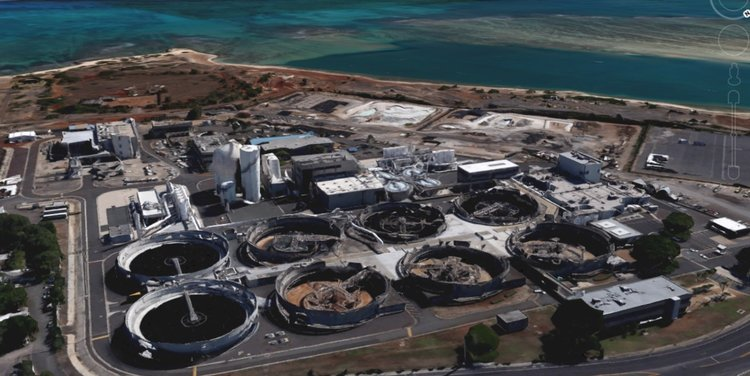
\includegraphics[width=3in]{figures/SIWWTP} \label{orgfe0a509} 
\par\end{center}
EnoQua Membrane Bioreactor 
\begin{center}
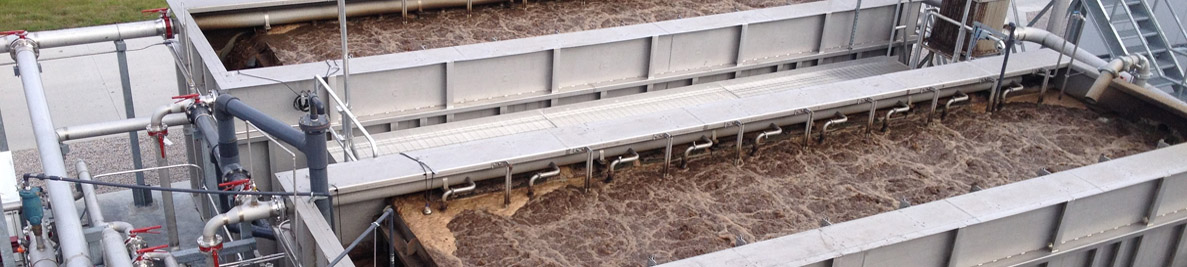
\includegraphics[width=3in]{figures/adi-mbr-p} \label{orgfe0a509} 
\par\end{center}

\end{frame}
%
\begin{frame}[label={sec:org3fde085}]{How to Reduce HF Fouling: Blowing → SHAKING}
\vspace{0.25cm}
 
\begin{columns}[]
% The "c" option specifies centered vertical alignment
% while the "t" option is used for top vertical alignment
\begin{column}{.45\textwidth} \centering 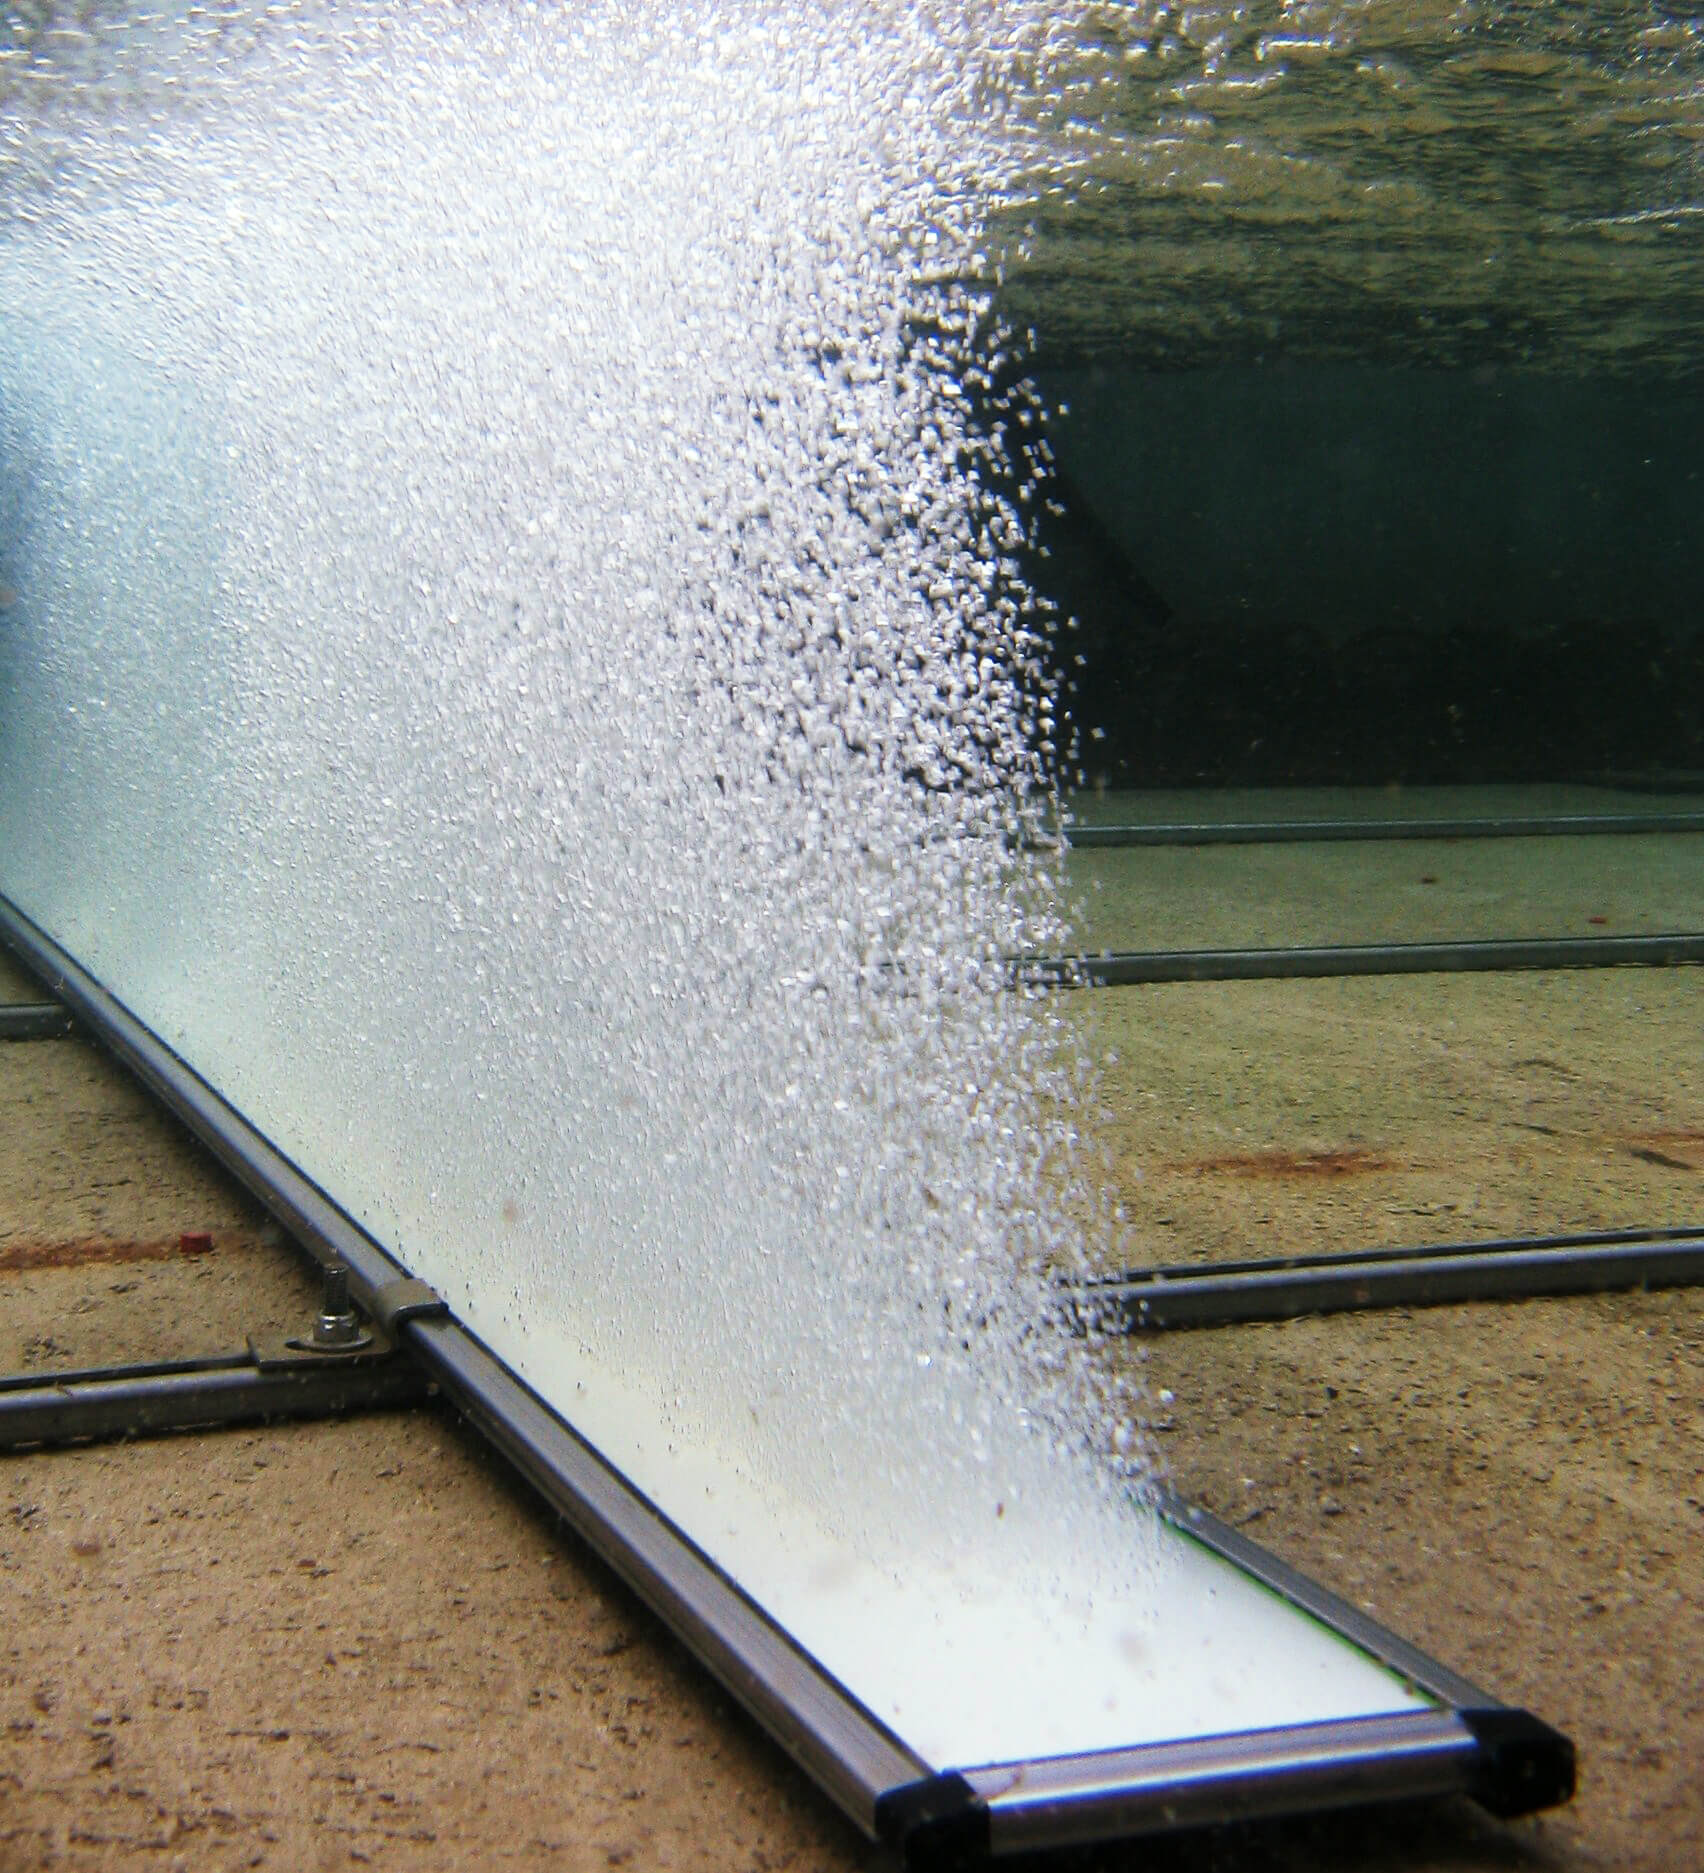
\includegraphics[height=1.75in]{figures/airdiffuser2} 

AERO% AEROSTRIP AERATORS
\end{column} \begin{column}{.45\textwidth} % Right column and width
\centering 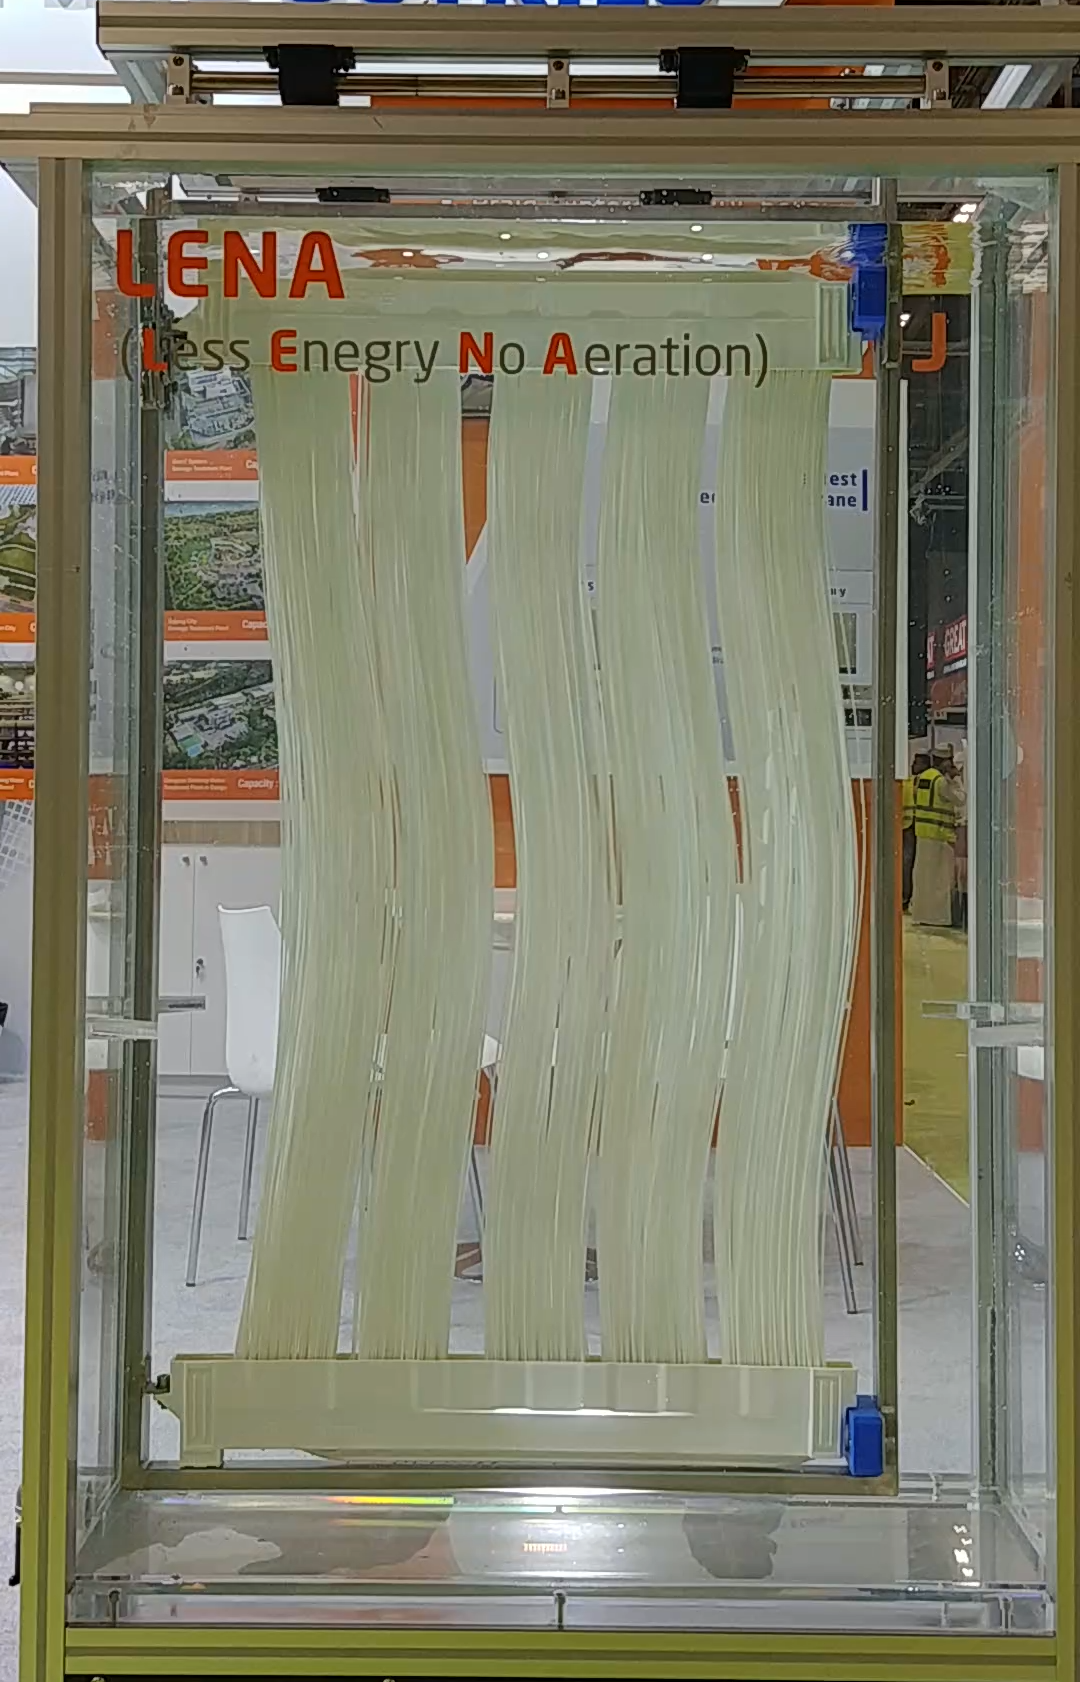
\includegraphics[height=1.75in]{figures/LENA-img_2018_04_29_18_45} 

Kolon, LENA \end{column} 
\end{columns}

\begin{itemize}
\item "\alert{Low Energy No Aeration}" (LENA) 
\begin{enumerate}
\item a new \emph{counter-intuitive} membrane technology: 
\item energy saving: $\approx$ 25\% 
\item shaking consumes less energy than blowing. 
\item \href{https://drive.google.com/file/d/1biSZK0caHFg7mzu3PPcHoZ9\%5C_O4z7kR4d/view?usp=sharing}{video 1}\&
\href{https://drive.google.com/file/d/1qSkZDnRfBLKfTKIlvScXDiLdXoNnRZLH/view?usp=sharing}{video 2}
\end{enumerate}
\end{itemize}
\end{frame}

\subsection{Research Task}

\label{sec:org9b61933} 
\begin{frame}[label={sec:orgcae7768}]{Does Dynamics of Hollow Fiber Follow Wave Equation? NO!}
\vspace{0.25cm}
 
\begin{columns}[c]
% The "c" option specifies centered vertical alignment
% while the "t" option is used for top vertical alignment
\begin{column}{.35\textwidth} \centering 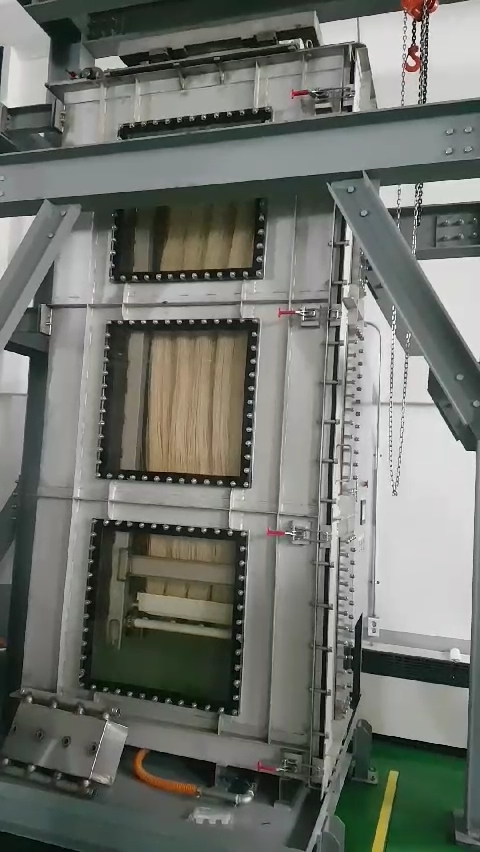
\includegraphics[height=2in]{figures/LENA-img_2018_05_10_14_30}
%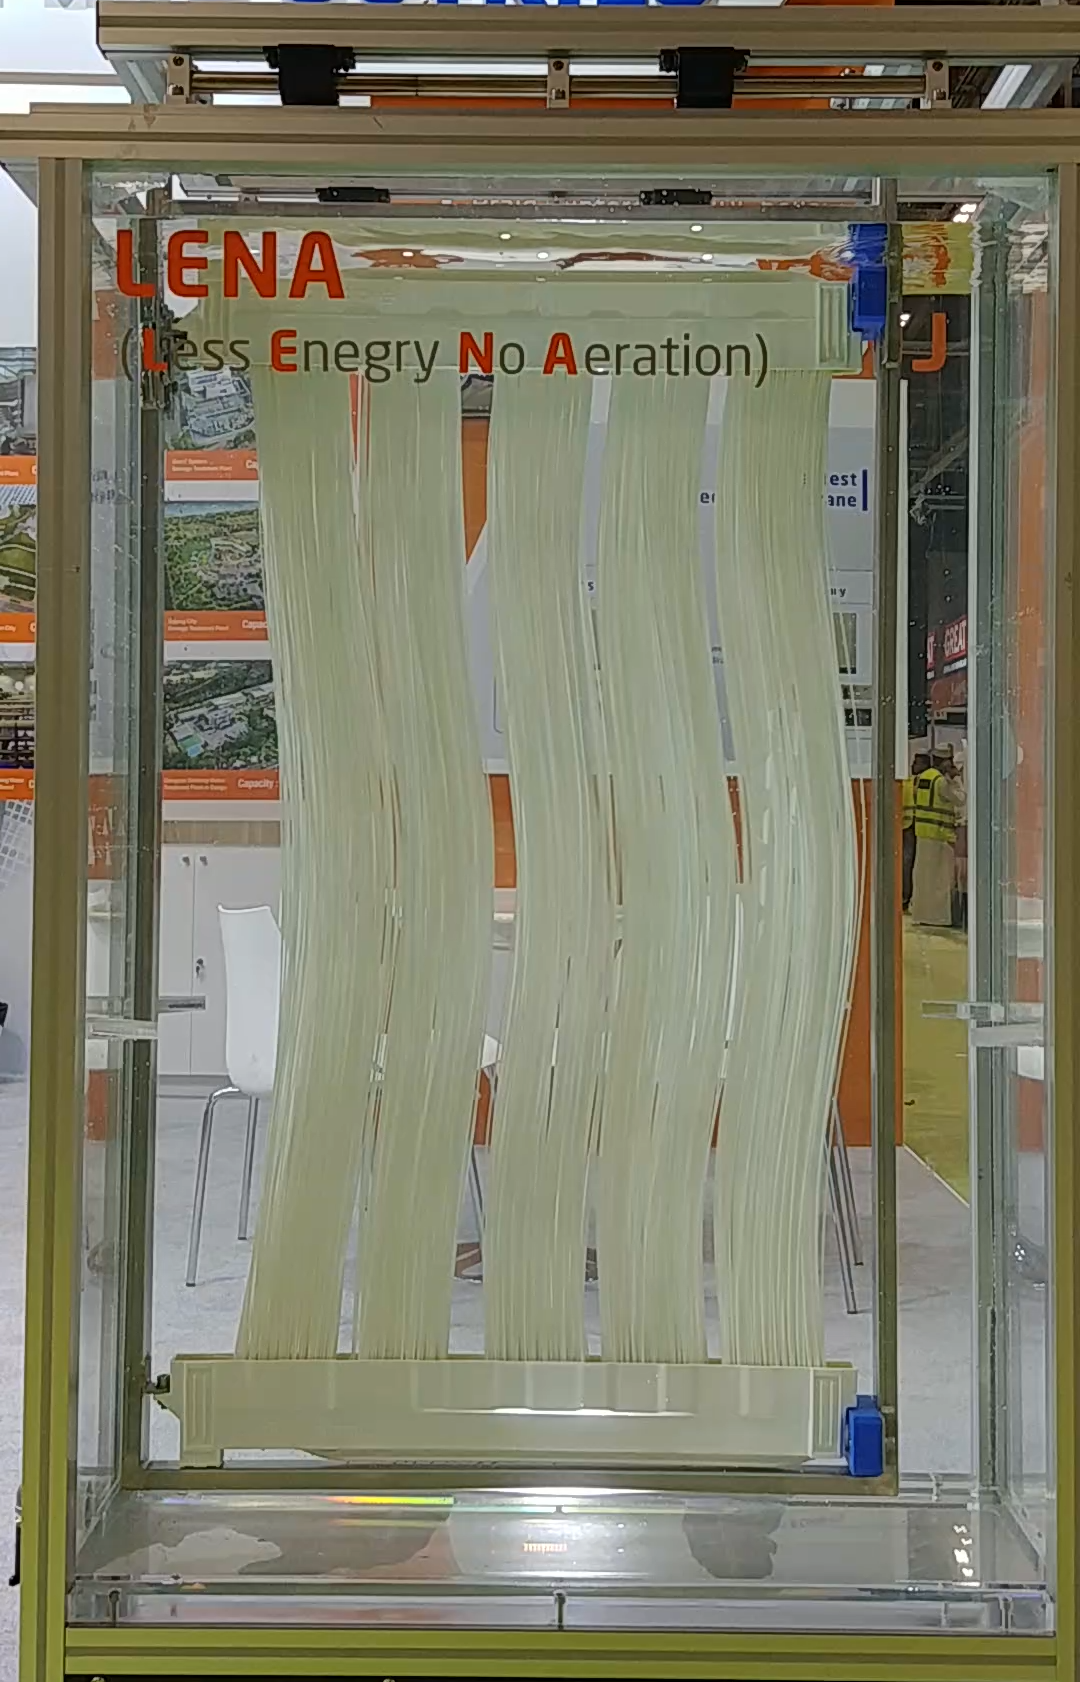
\includegraphics[height=2in]{figures/LENA-img_2018_04_29_18_45.png}
%#

(a) LENA \end{column} \begin{column}{.55\textwidth} % Right column and width
\centering 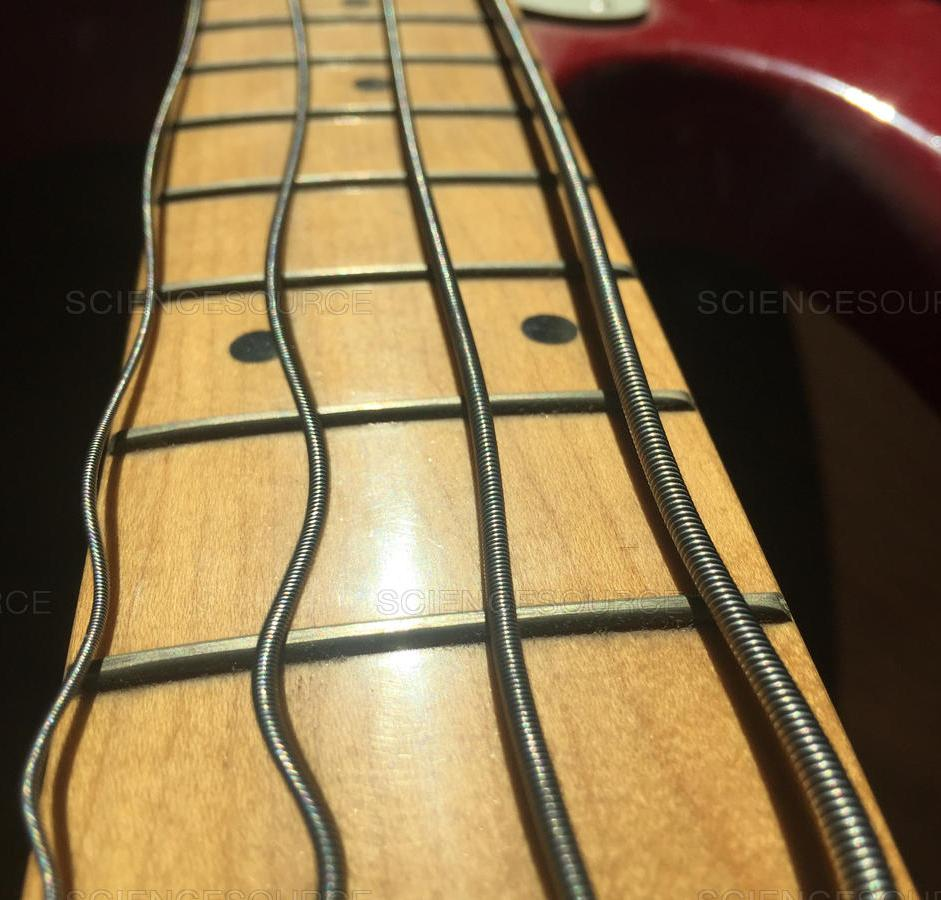
\includegraphics[height=2in]{figures/vib-guitar-strings} 

(b) Vibrating guitar strings \end{column} 
\end{columns}

In (b), string image\footnote{\url{https://www.sciencesource.com/archive/Vibrations-in-Guitar-Strings-SS2781967.html}} 
\end{frame}

\section{Theory and Simulations}

\label{sec:orgf43736a} 

\subsection{Equivalent Sphere}

\label{sec:orgfd2df02} 
\begin{frame}[label={sec:org106a788}]{Hollow Fiber Segment vs. Equivalent Sphere}
\vspace{0.25cm}
 
\begin{columns}[c]
% The "c" option specifies centered vertical alignment
% while the "t" option is used for top vertical alignment
\begin{column}{.45\textwidth} \centering 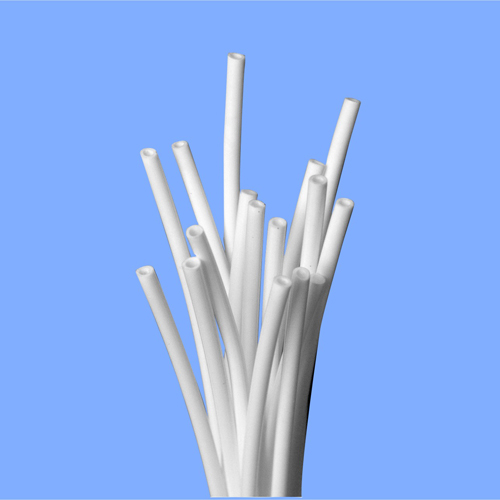
\includegraphics[width=1.5in]{figures/hydroblue}

(a) fiber bundle 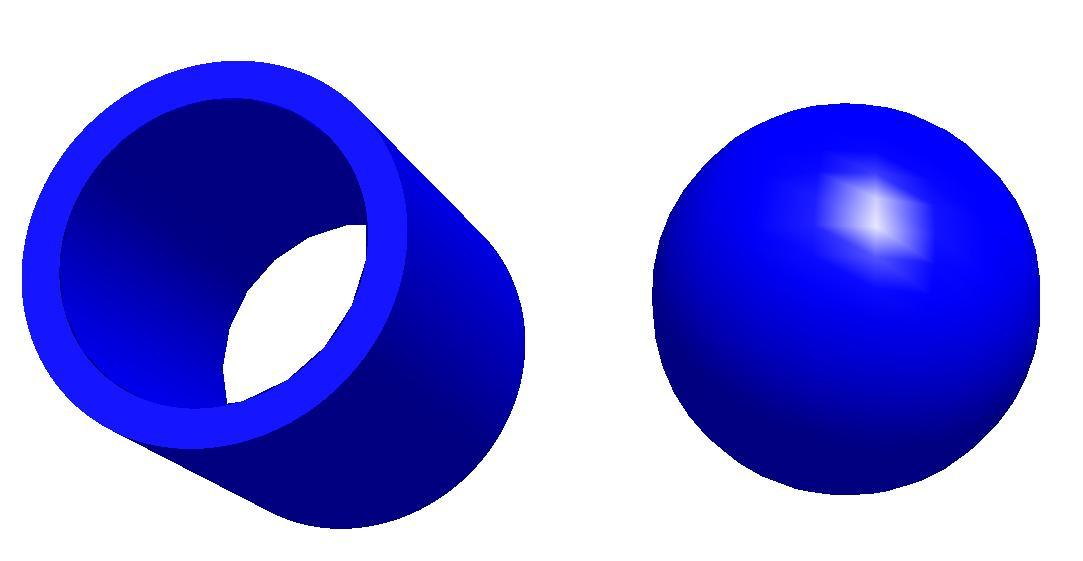
\includegraphics[width=1.5in]{figures/equiv-sphere}

(b) fiber seg. \& equiv. sphere \end{column} \begin{column}{.45\textwidth}
% Right column and width
\centering 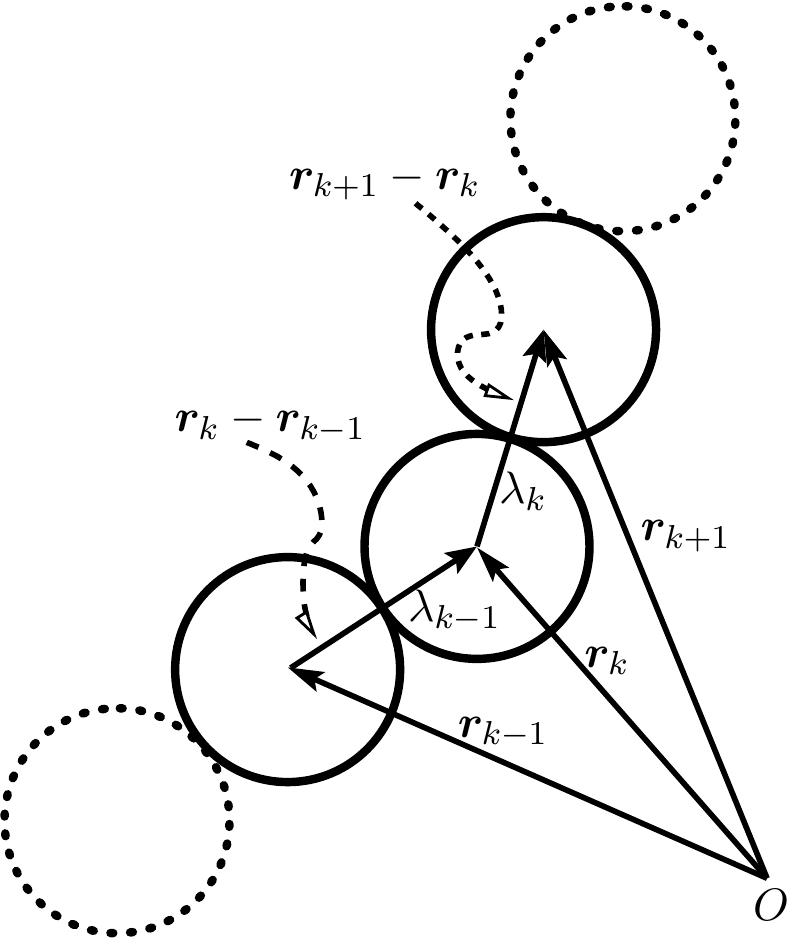
\includegraphics[height=2in]{figures/fig-trimer-rot-crop2-1}

(c) fiber as linked sphers \end{column} 
\end{columns}

\end{frame}
%
\begin{frame}[label={sec:org16e0822}]{Hollow Fiber Segment vs. Equivalent Sphere (cont'd)}
\vspace{0.25cm}
 
\begin{columns}[c]
% The "c" option specifies centered vertical alignment
% while the "t" option is used for top vertical alignment
\begin{column}{.45\textwidth} \centering 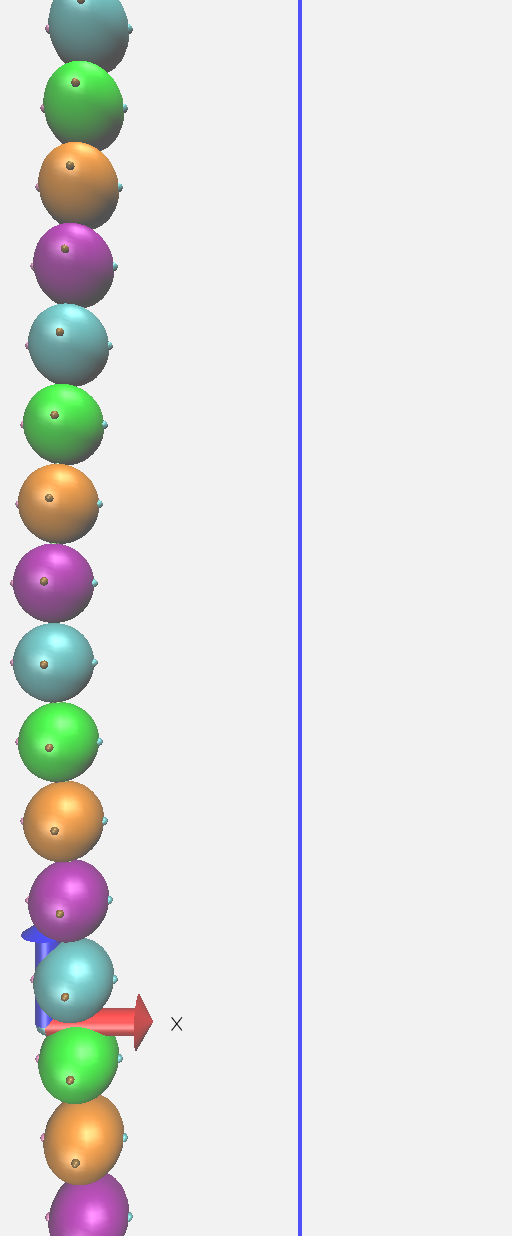
\includegraphics[height=2.25in]{figures/fig-chain-100-spheres-nearview-t00}

%(a) fiber bundle
\end{column} \begin{column}{.45\textwidth} % Right column and width
\centering 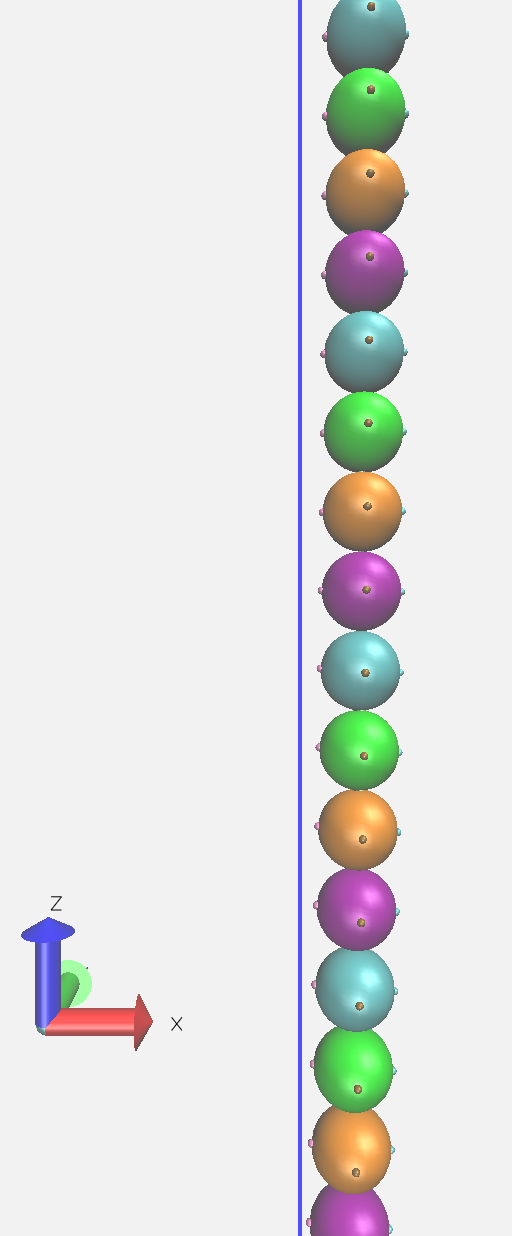
\includegraphics[height=2.25in]{figures/fig-chain-100-spheres-nearview-t24}

%(c) fiber as linked sphers
\end{column} 
\end{columns}

\begin{itemize}
\item Sphere colors are just for visualization 
\item Black dots (6 per sphere) is to see sphere rotation. 
\end{itemize}
\end{frame}

\subsection{Constraint Dynamics}

\label{sec:org16e9670} 
\begin{frame}[label={sec:org537322b}]{Theoretical approaches}
\begin{block}{Holonomic constraints: center-to-center distance}
\begin{equation}
\sigma_{k}=\left(\bm{r}_{k}-\bm{r}_{k+1}\right)^{2}-d_{k,k+1}^{2}=0
\end{equation}
\end{block}
\end{frame}
%
\begin{block}{Non-Holonomic constraints: position-velocity orthogonality}
\begin{equation}
\left(\bm{r}_{k}-\bm{r}_{k+1}\right)\cdot\left(\bm{v}_{k}-\bm{v}_{k+1}\right)=0\label{eq:orthogonal}
\end{equation}
\end{block}
%
\begin{block}{Total Force = External + Internal}
\begin{enumerate}
\item External: 
\begin{enumerate}
\item gravitational force (vector-wise) 
\begin{enumerate}
\item hydrodynamic force/torque (tensor-wise) 
\end{enumerate}
\item Internal 
\begin{enumerate}
\item holonomic 
\item non-holonomic constraint forces 
\end{enumerate}
\end{enumerate}
\end{enumerate}
\end{block}
%
\begin{frame}[label={sec:org835dbac}]{Constraint Forces}
\begin{block}{Holonomic Constraint Force on sphere $k$}
\begin{align}
m_{k}\bm{a}_{k}^{c} & =\lambda_{k-1}\left(\bm{r}_{k-1}-\bm{r}_{k}\right)-\lambda_{k}\left(\bm{r}_{k}-\bm{r}_{k+1}\right)\label{eq:cstr-frc}
\end{align}
where $\lambda$ is the Lagrange multiplier, to be instantaneously
updated as responding to non-internal forces. 
\end{block}
\end{frame}
%
\begin{block}{Non-holonomic Constraint Force on sphere $k$}
\begin{equation}
m_{k}\bm{a}_{k}^{n}=\kappa_{k-1}\left(\bm{r}_{k-1}-\bm{r}_{k}\right)-\kappa_{k}\left(\bm{r}_{k}-\bm{r}_{k+1}\right)
\end{equation}
has the same mathematical form, but $\kappa\ne\lambda$. 
\end{block}
%
\begin{block}{Constraint Dynamics Simulation}
\begin{itemize}
\item How to efficiently calculate/update $\lambda$ and $\kappa$ for evol. 
\end{itemize}
\end{block}
%
\begin{frame}[label={sec:org88c4e05}]{External Forces}
\begin{block}{Gravitational + Buoyant Forces}
\begin{equation}
\bm{F}_{j}^{G}=\Delta m_{j}\bm{g}
\end{equation}
where $\Delta m_{j}=m_{j}-m_{f}$, and \$m\_\{f\}is the mass of fluid. 
\end{block}
\end{frame}
%
\begin{block}{Hydrodynamic Forces/Torques ← Stokesian Dynamics}
\begin{equation}
\left[\begin{array}{c}
\bm{U}^{\infty}-\bm{v}_{j}\\
\Omega^{\infty}-\bm{\omega}_{j}\\
\bm{E}^{\infty}\phantom{--\bm{0}_{i}}
\end{array}\right]=\sum_{k=1}^{N_{p}}\left[\begin{array}{ccc}
\bm{a}_{jk} & \tilde{\bm{b}}_{jk} & \tilde{\bm{b}}_{jk}\\
\bm{b}_{jk} & \bm{c}_{jk} & \tilde{\bm{h}}_{jk}\\
\bm{g}_{jk} & \bm{h}_{jk} & \bm{m}_{jk}
\end{array}\right]\cdot\left[\begin{array}{c}
\bm{F}_{k}^{H}\\
\bm{T}_{k}^{H}\\
\bm{S}_{k}^{H}
\end{array}\right]\label{eq:grandMobil}
\end{equation}
where $\left[\bm{F}_{k}^{H},\bm{T}_{k}^{H},\bm{S}_{k}^{H}\right]^{\mathrm{tr}}$
is hydrodynamic force, torque, stresslet vectors, in an ambient flow
field: 
\begin{equation}
\bm{v}^{D}\left(\bm{r}_{j}\right)=\bm{U}^{\infty}+\bm{\Omega}^{\infty}\times\bm{x}+\bm{E}^{\infty}:\bm{x}\quad\mathrm{for}\quad\bm{x}\in S_{j}
\end{equation}
\end{block}

\subsection{Dissipative Hydrodynamics (DHD)}

\label{sec:org1133e0a} 
\begin{frame}[label={sec:org869a0d6}]{Grand Governing Equation for $N_{p}$ Connected Spheres}
\ldots{} requiring to solve a linear system of $11N_{p}\times11N_{p}$
matrix. 
\begin{equation}
\left[\begin{array}{cc}
m_{k} & 0\\
0 & I_{k}
\end{array}\right]\left[\begin{array}{c}
\bm{a}_{k}\\
\bm{\alpha}_{k}
\end{array}\right]=\left[\begin{array}{c}
\bm{F}_{k}^{H}\\
\bm{T}_{k}^{H}
\end{array}\right]+\left[\begin{array}{c}
\bm{F}_{k}^{E}\\
0
\end{array}\right]+\left[\begin{array}{c}
\bm{F}_{k}^{C}\\
0
\end{array}\right]\label{eq:goveq}
\end{equation}
\begin{itemize}
\item If $N_{p}=1,000$, the no. of element = 121,000,000 
\item Memory = element no. times 8 byte → $\approx$1.0 GB. 
\end{itemize}
\begin{center}
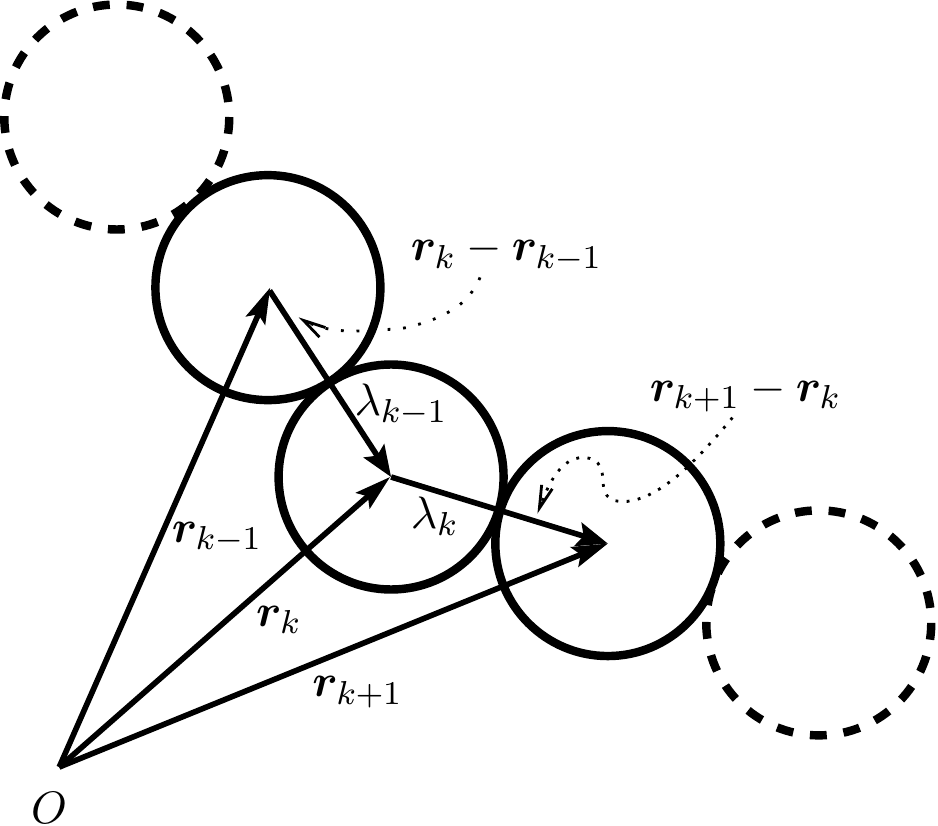
\includegraphics[width=2in]{figures/fig-trimer-crop-1} \label{orgec93873} 
\par\end{center}
\end{frame}

\section{Results and Discussions}

\label{sec:orga751918} 

\subsection{Hollow Fiber Specifications}

\label{sec:org222bee5} 
\begin{frame}[label={sec:org5262d8d}]{Simulation parameters: rack and fibers}

\begin{table}[H]
\centering{}%
\begin{tabular}{|l|l|r|r|}
\hline 
 & Variables  & Value  & Value\tabularnewline
\hline 
\hline 
\multirow{1}{*}{} & Fiber length {[}mm{]}, $L_{f}$  & 1000  & 2000\tabularnewline
\hline 
 & Number of spheres, $N_{p}$  & 500  & 1000\tabularnewline
\hline 
 & Stack height {[}mm{]}, $H=L_{f}/(1+R_{st})$  & 998  & 1996\tabularnewline
\hline 
 & Oscillation Amplitude {[}mm{]}, $A$  & 6.0  & 12.0\tabularnewline
\hline 
 & Oscillation frequency {[}Hz{]}, $\omega$  & 0.46  & 0.46\tabularnewline
\hline 
\end{tabular}\caption{\label{tab:stack-parameters}Simulation parameters of the rack and
fibers, where the oscillation amplitude is calculated as $A=0.06\,L_{f}$
and the stack ratio of $R_{\mathrm{st}}=0.2\,\%$ is used. Based on
the common frequency, the period of the rack oscillation is calculated
as $\tau=2.1739$ s.}
\end{table}
\end{frame}
%
\begin{frame}[label={sec:org82e97a1}]{Simulation parameters: rack and fibers}
\begin{table}[H]
\centering{}%
\begin{tabular}{|l|l|r|r|}
\hline 
 & Variables  & PVDF  & PET\tabularnewline
\hline 
\hline 
\multirow{1}{*}{} & Solid density, $\rho_{s}$  & 1.780  & 1.380\tabularnewline
\hline 
 & Outer diameter {[}mm{]}, $d_{o}=2a_{f}$  & 2.000  & 2.000\tabularnewline
\hline 
 & Inner diameter {[}mm{]}, $d_{i}=2a_{f}^{\prime}$  & 1.600  & 0.700\tabularnewline
\hline 
 & Thickness {[}mm{]}, $a_{f}-a_{^{\prime}f}$  & 0.200  & 0.650\tabularnewline
\hline 
 & Porosity {[}-{]}, $\epsilon$  & 0.650  & 0.650\tabularnewline
\hline 
 & Water-filled fiber material density, $\bar{\rho}_{f}$  & 1.273  & 1.133\tabularnewline
\hline 
 & Mass of cylindrical segment {[}mg{]}, $m_{s}$  & 6.901  & 7.017\tabularnewline
\hline 
\multirow{1}{*}{} & Volume {[}mm\textsuperscript{3}{]}  & 4.189  & 4.189\tabularnewline
\hline 
 & Specific gravity {[}--{]}, $s_{g}$  & 1.647  & 1.675\tabularnewline
\hline 
\end{tabular}\caption{\label{tab:HF-parameters}Simulation parameters of the rack and fibers
and equivalent spheres, made of polyvinylidene fluoride (PVDF) and
polyethylene terephthalate (PET).}
\end{table}
\end{frame}

\subsection{Chain Dynamics Animation}

\label{sec:org544d6d4} 
\begin{frame}[label={sec:orgd5aa4b4}]{Snapshots during 6 quarter periods}
\vspace{0.25cm}
 
\begin{columns}[c]
% The "c" option specifies centered vertical alignment
% while the "t" option is used for top vertical alignment
\begin{column}{.25\textwidth} \centering 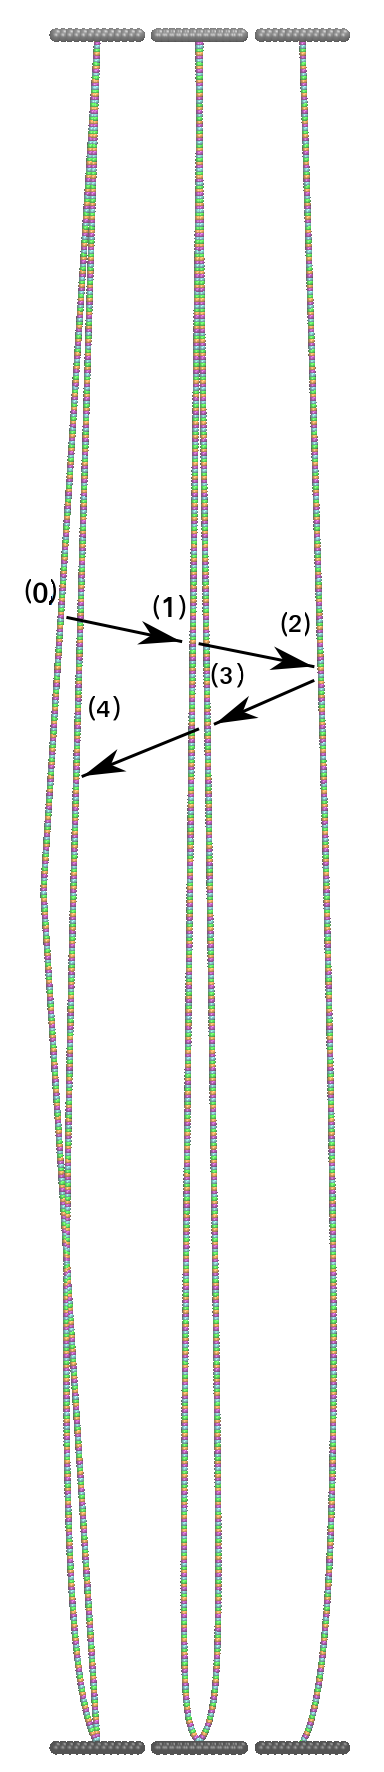
\includegraphics[height=2.75in]{figures/pvdf_short_time_shots_1p5zoom_crop_anno_arrow2} 

\end{column} \begin{column}{.65\textwidth} % Right column and width
Periodic motion 
\begin{itemize}
\item 0: initial rightmost position 
\item 1: $t=\tau_{1/4}$ after a \textbf{quarter period} 
\item 2: $t=2\tau_{1/4}$ after two quarter period 
\item 3: $t=3\tau_{1/4}$ after a half period 
\item 4: $t=4\tau_{1/4}$ after a full period 
\item 5: $t=5\tau_{1/4}$ after 1.25 period 
\item 6: $t=6\tau_{1/4}$ after 1.50 period 
\end{itemize}
where $\tau_{1/4}=\tau/4$ is a quarter period. \end{column} 
\end{columns}

\end{frame}

\subsection{Constraint Force on Short Chain}

\label{sec:orge853c19} 
\begin{frame}[label={sec:org9ecb48b}]{{[}Short Chain{]} Constraint Forces in $x-$ Direction}
\begin{itemize}
\item Backward \& forward constraint forces: anti-symmetric. 
\item Near $z=l_{f}/4$, i.e., 25\% height, almost $F_{x}^{c}\to0$ {[}nN{]}. 
\end{itemize}
%\vspace{0.25cm}
\begin{columns}[c]
% The "c" option specifies centered vertical alignment
% while the "t" option is used for top vertical alignment
\begin{column}{.45\textwidth} \centering 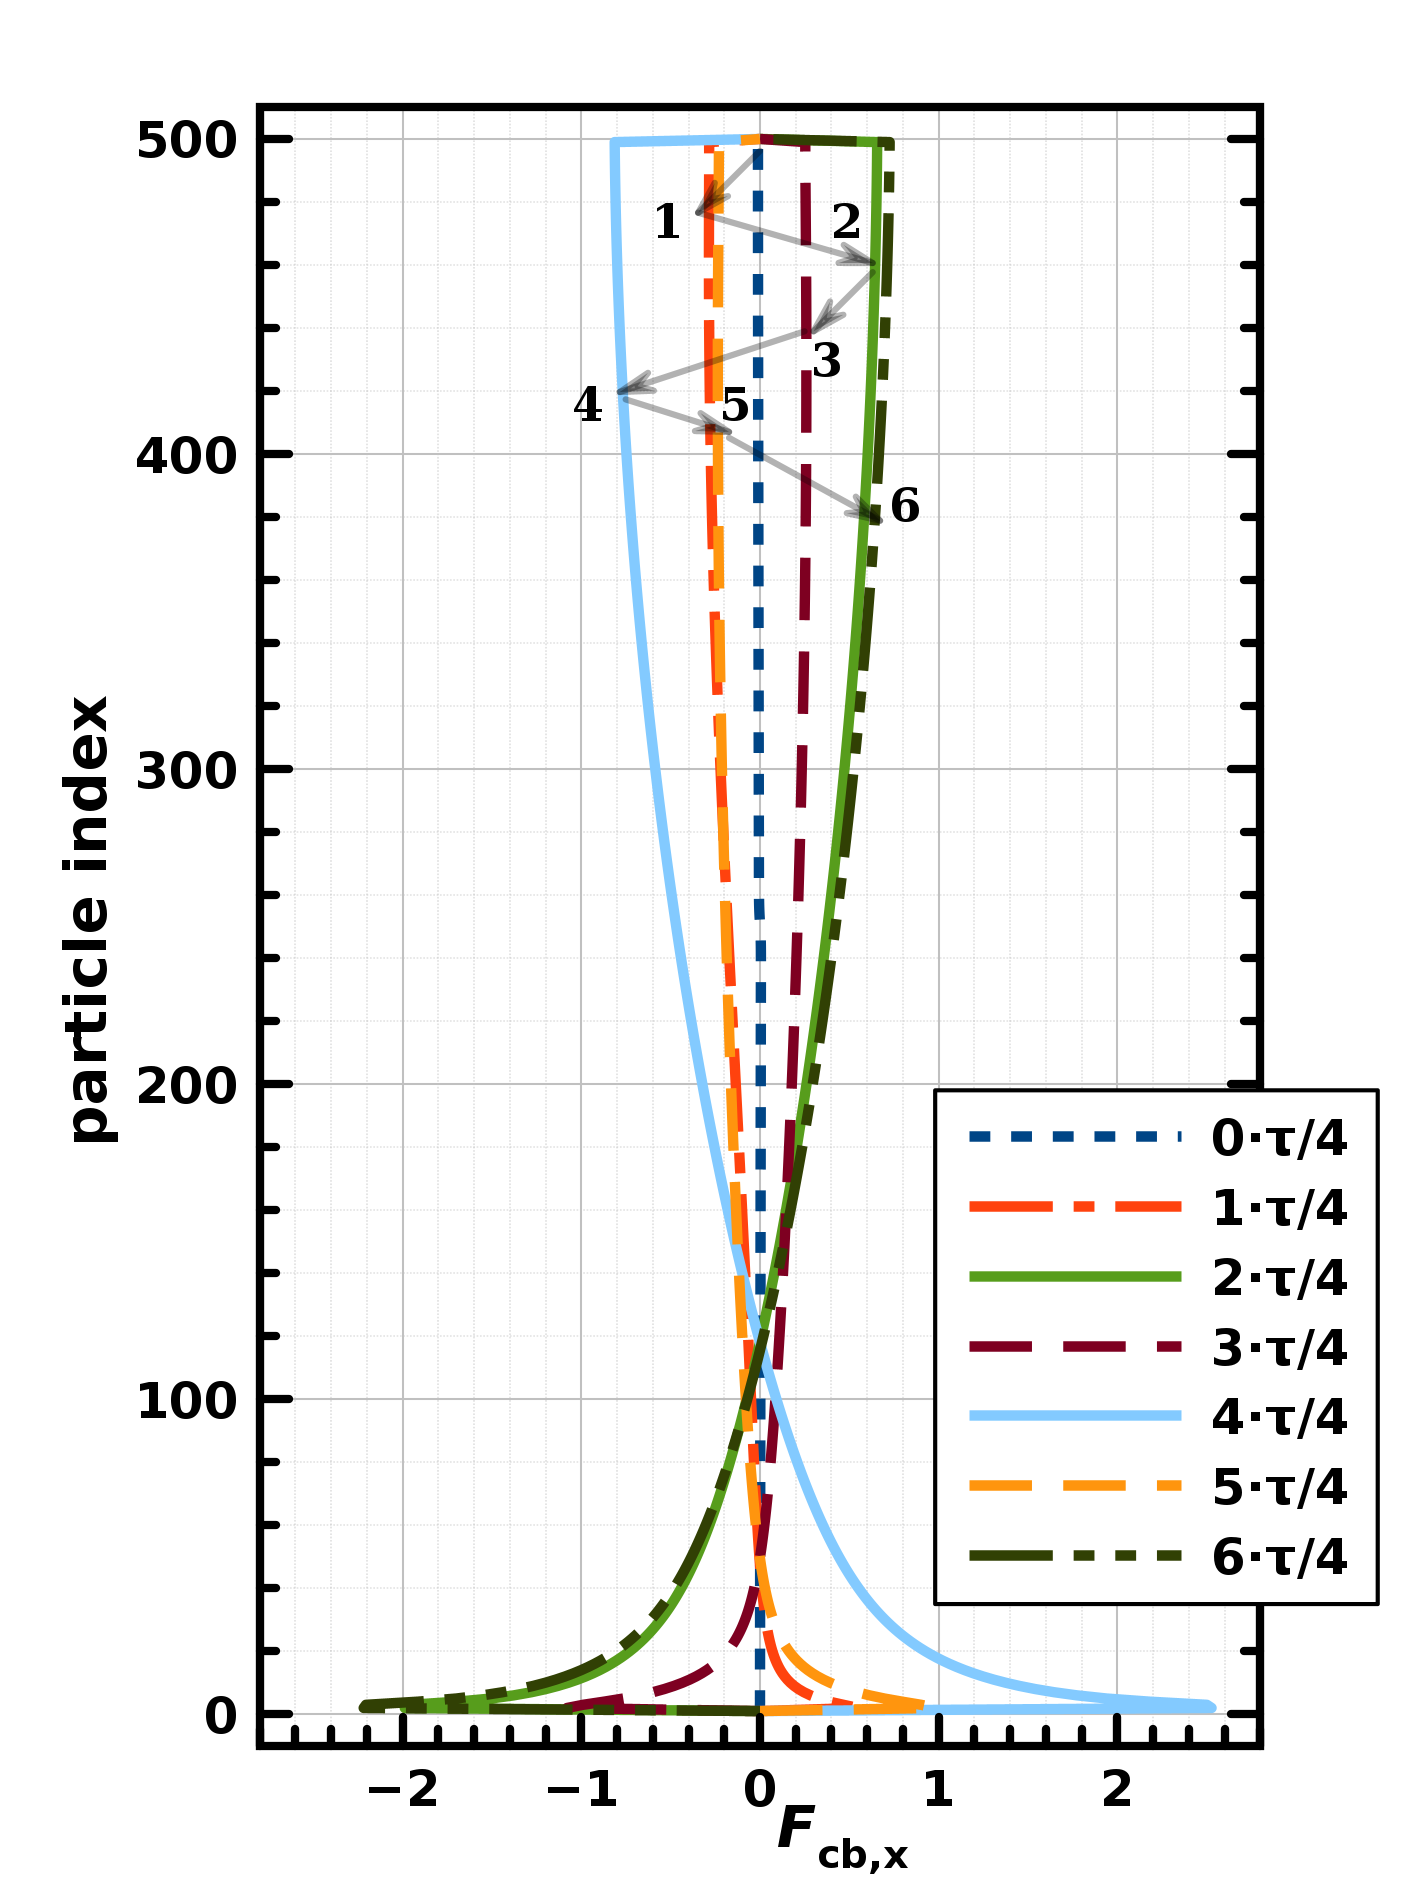
\includegraphics[width=1.75in]{figures/cXpvdf500FC1}

\end{column} \begin{column}{.45\textwidth} % Right column and width
\centering 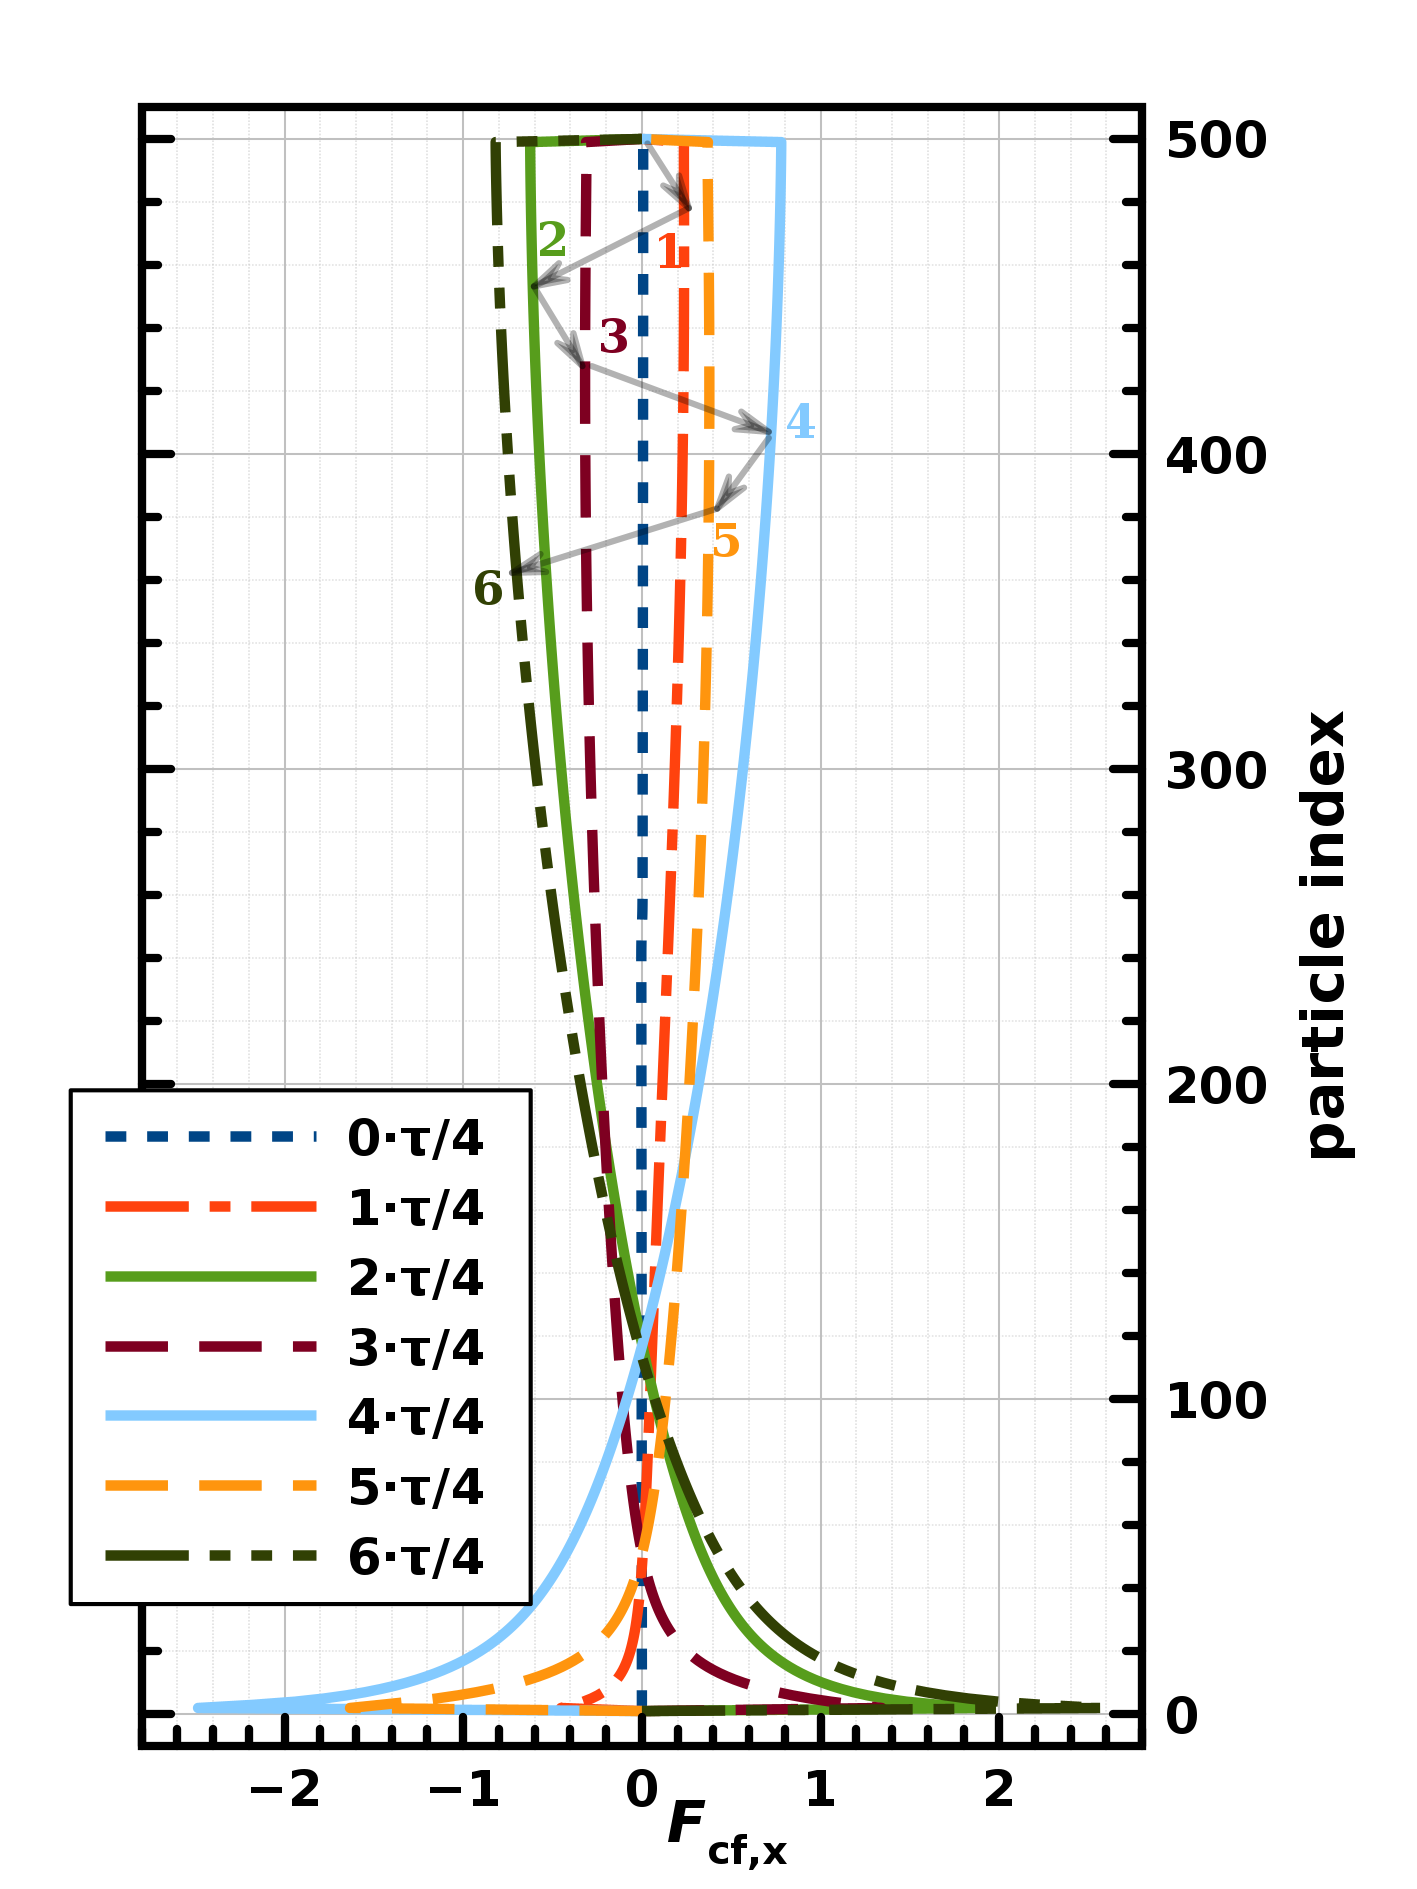
\includegraphics[width=1.75in]{figures/cXpvdf500FC2}

\end{column} 
\end{columns}

\end{frame}
%
\begin{frame}[label={sec:orgccef4ab}]{{[}Short Chain{]} Constraint Forces in $z-$ Direction}
\begin{itemize}
\item $F_{z}^{c}$ is about 10 times stronger than $F_{x}^{c}$ {[}nN{]}. 
\item Anti-symmetry appears, but not perfect. 
\end{itemize}
\begin{columns}[c]
% The "c" option specifies centered vertical alignment
% while the "t" option is used for top vertical alignment
\begin{column}{.45\textwidth} \centering 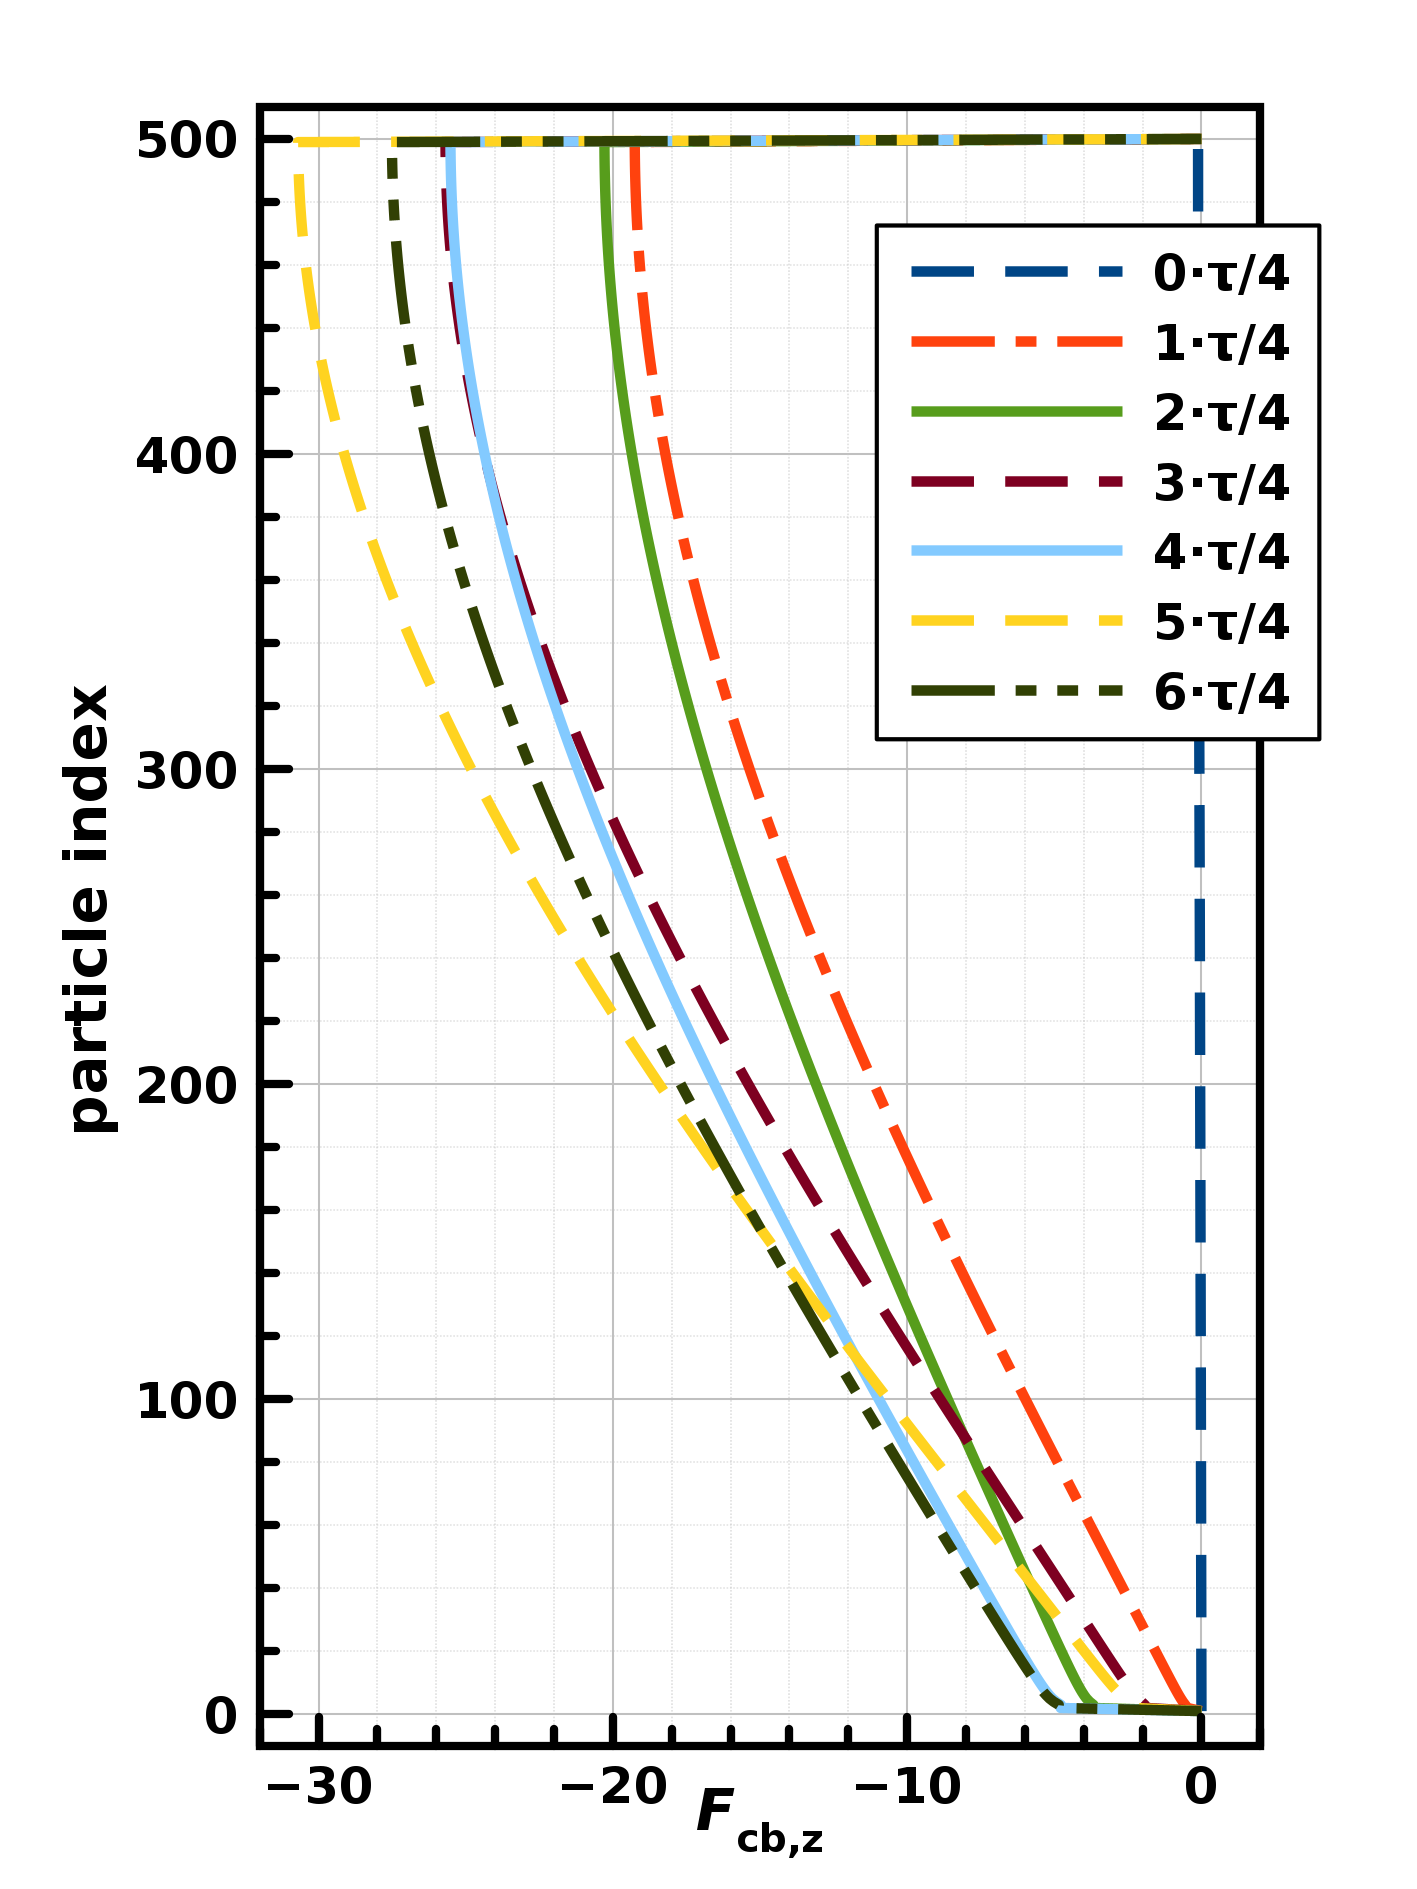
\includegraphics[width=1.75in]{figures/cZpvdf500FC1}

\end{column} \begin{column}{.45\textwidth} % Right column and width
\centering 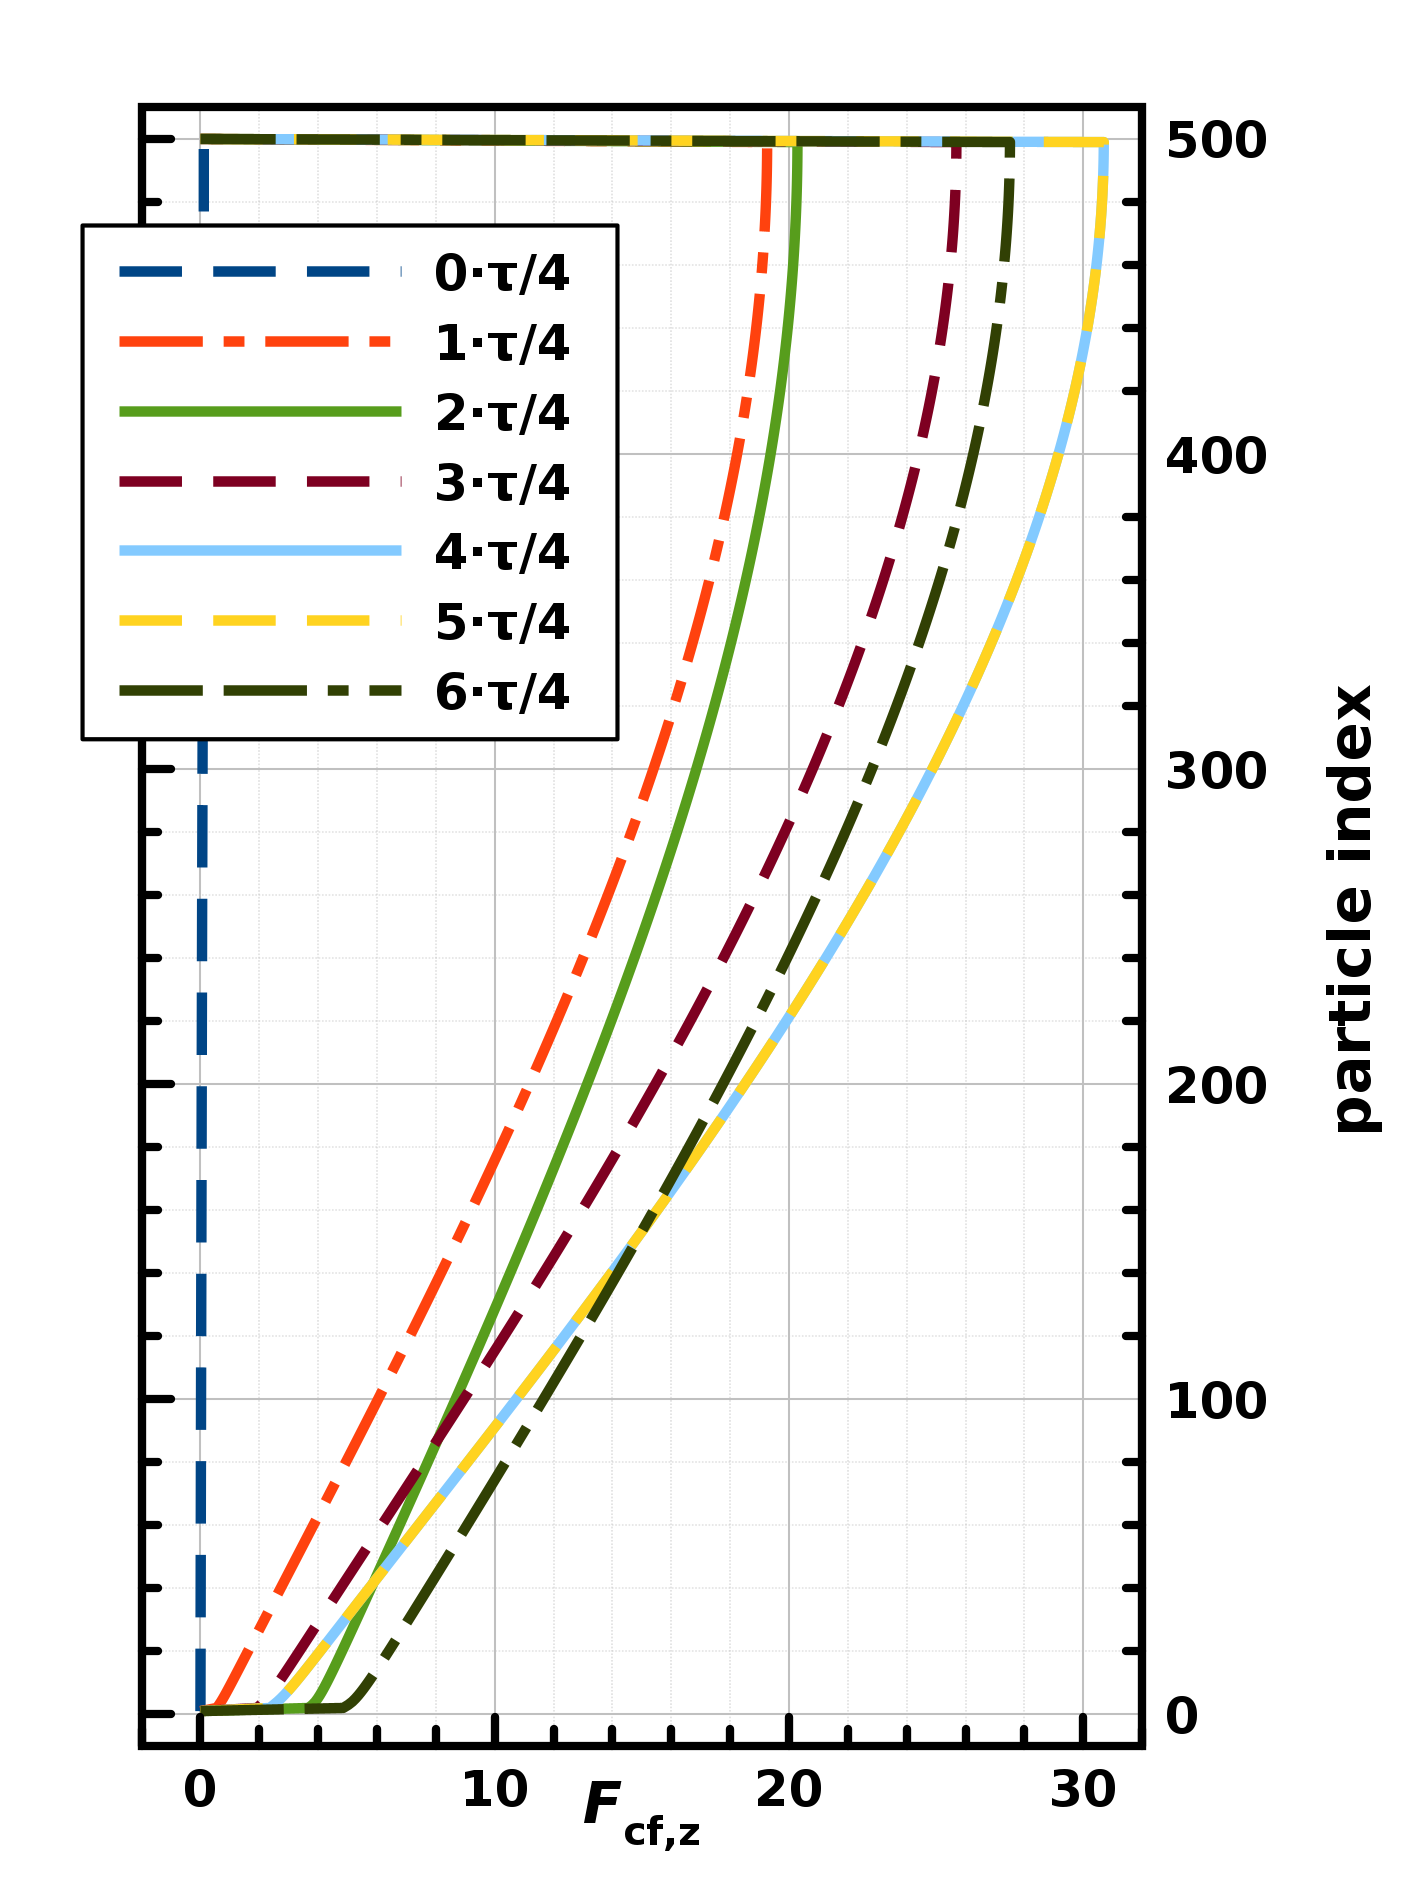
\includegraphics[width=1.75in]{figures/cZpvdf500FC2}

\end{column} 
\end{columns}

\end{frame}
%
\begin{frame}[label={sec:orgb590468}]{{[}Short Chain{]} Total Force in $x-$ and $z-$ Direction}
\begin{itemize}
\item The net total forces {[}$\mu{\rm {N}}${]} exerted mostly near the
bottom. 
\item Bottom and top segments can be mechanically reinforced. 
\end{itemize}
\begin{columns}[c]
% The "c" option specifies centered vertical alignment
% while the "t" option is used for top vertical alignment
\begin{column}{.45\textwidth} \centering 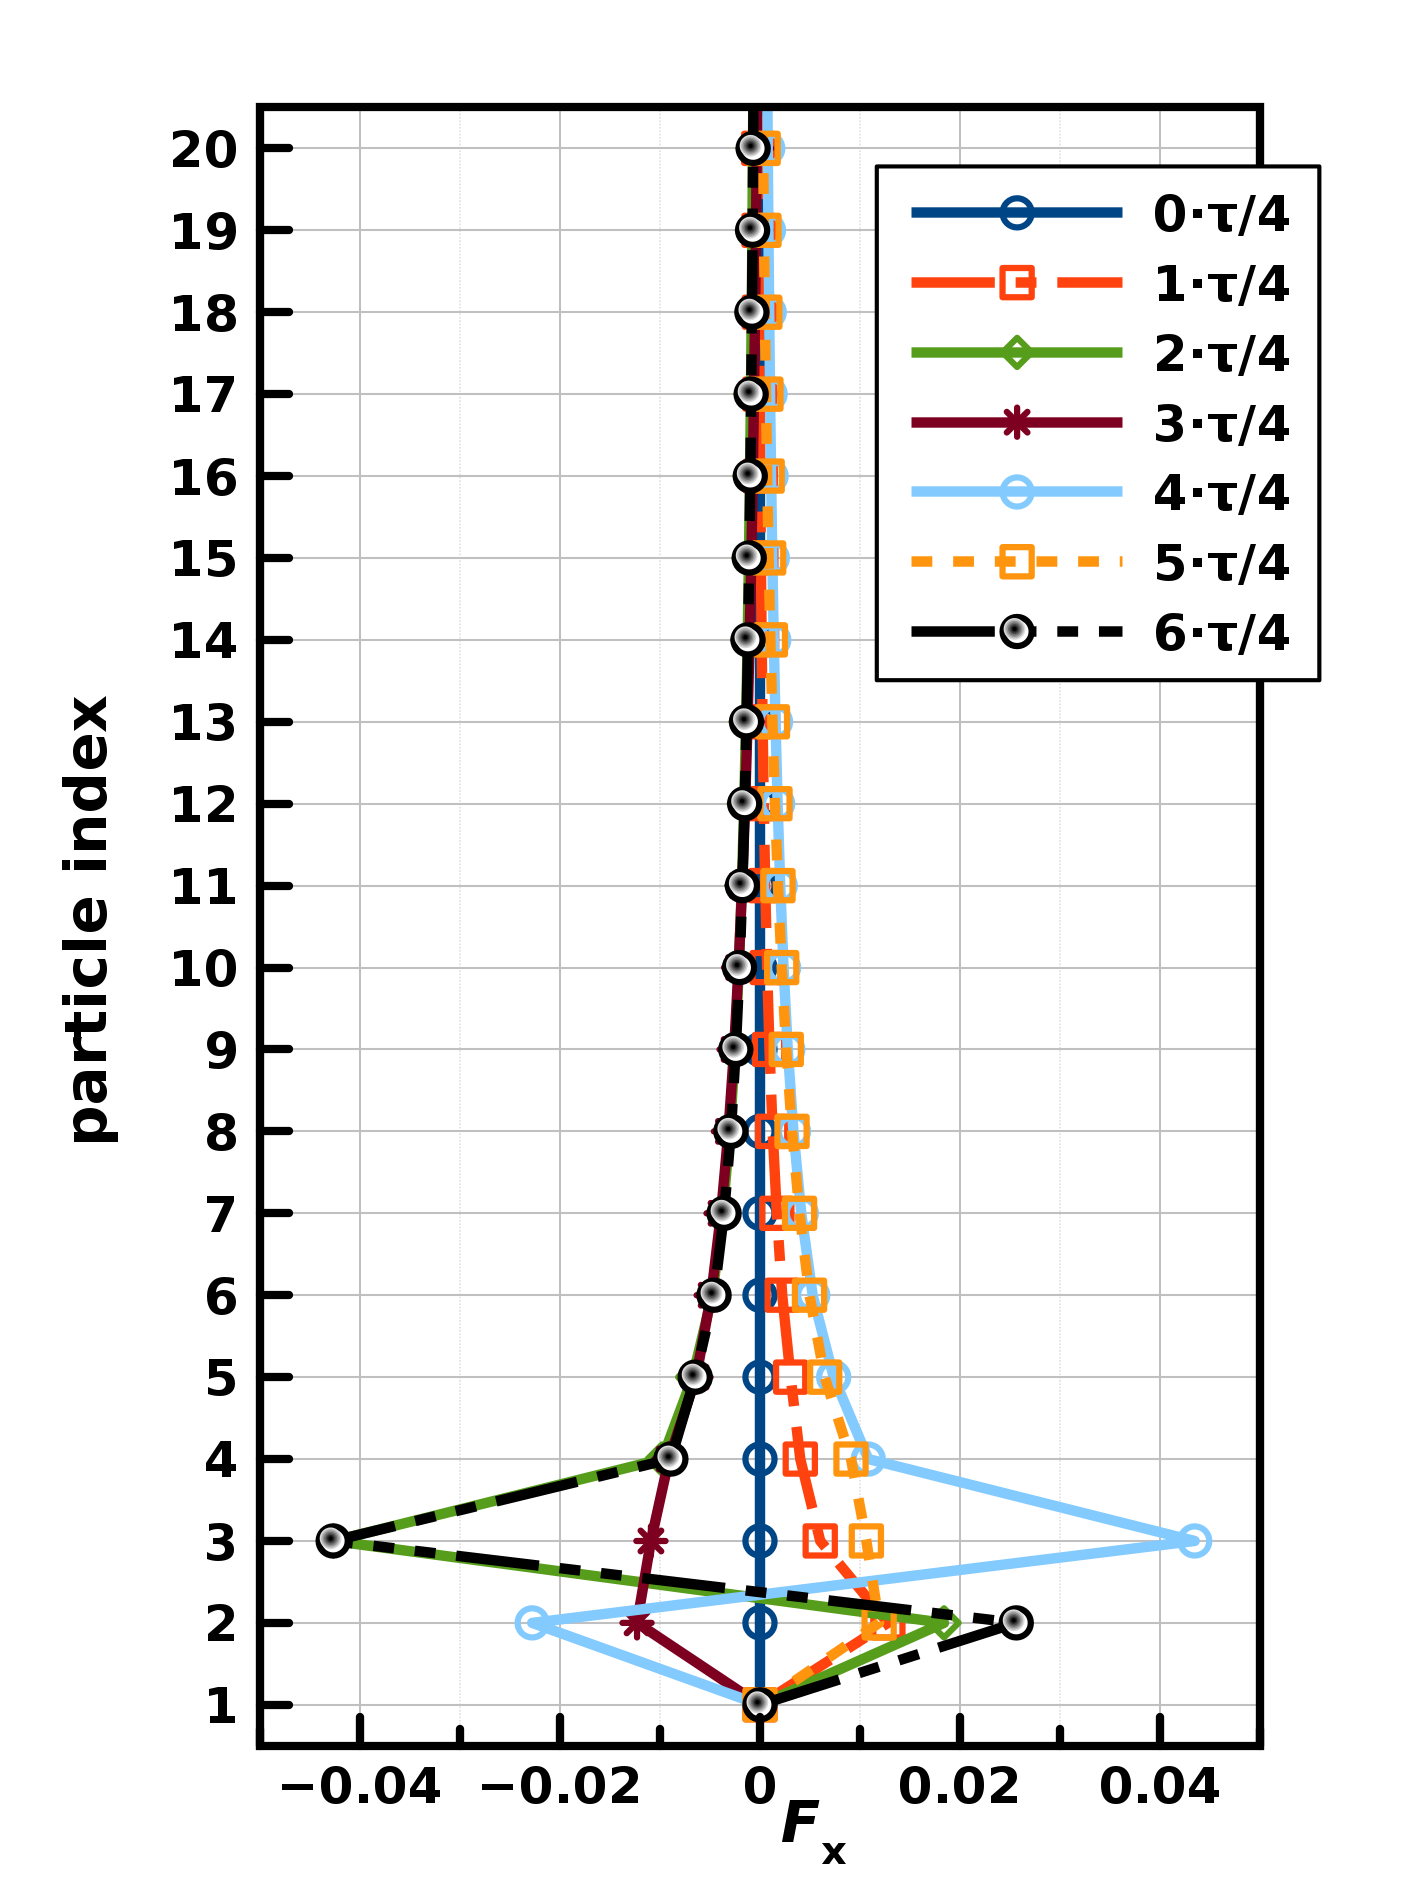
\includegraphics[width=1.75in]{figures/cXpvdf500FTS}

\end{column} \begin{column}{.45\textwidth} % Right column and width
\centering 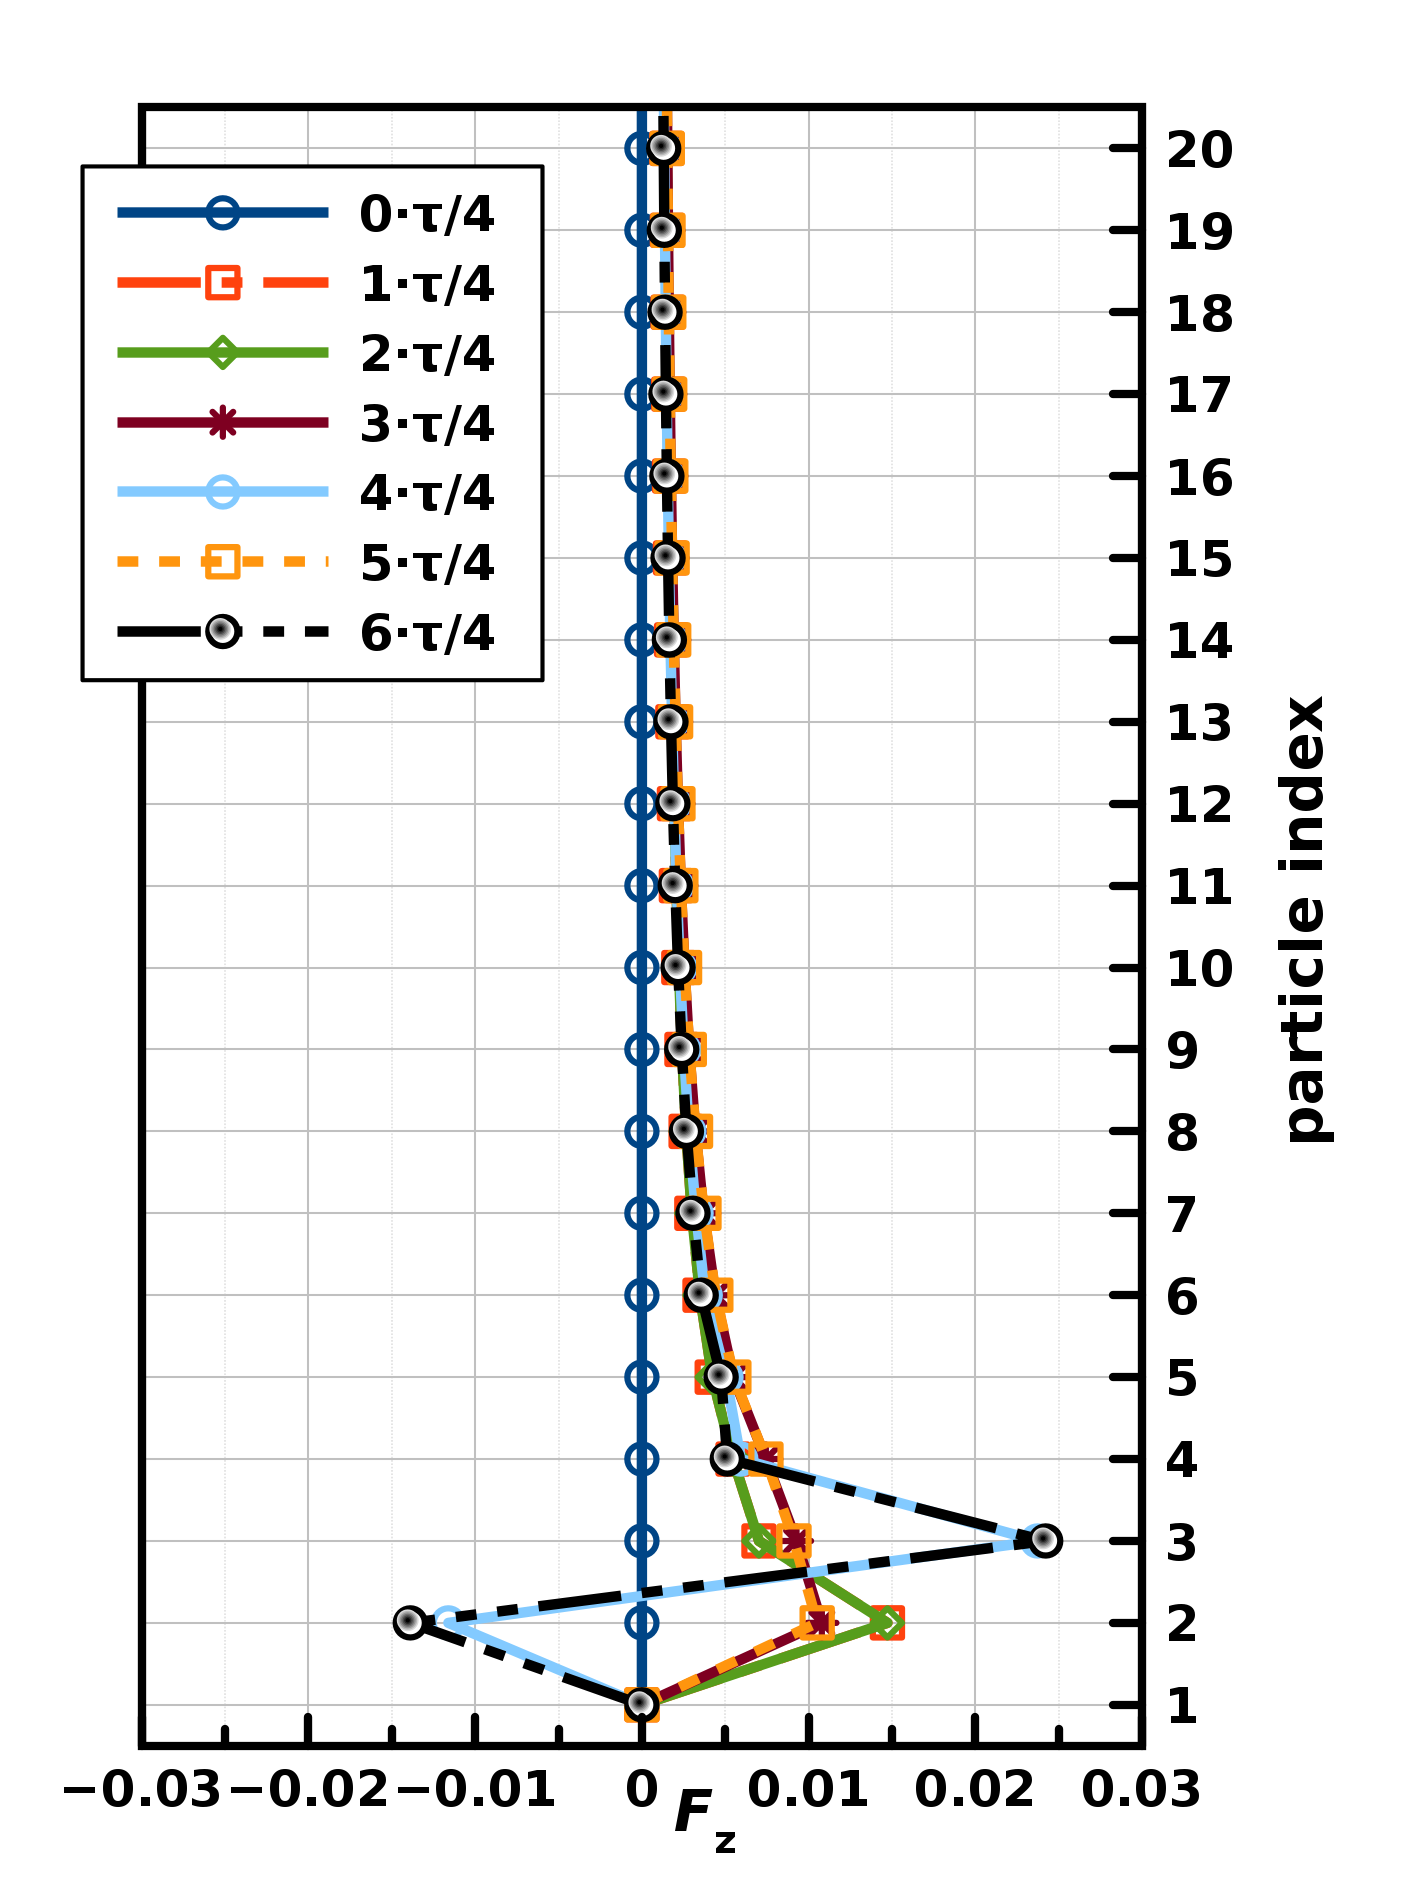
\includegraphics[width=1.75in]{figures/cZpvdf500FTS}

\end{column} 
\end{columns}

\end{frame}

\subsection{Constraint Force on Long Chain}

\label{sec:org57f7451} 
\begin{frame}[label={sec:orgf336b32}]{{[}Long Chain{]} Constraint Forces in $x-$ Direction}
\begin{itemize}
\item The zero-force {[}nN{]} zone becomes vague. 
\end{itemize}
\begin{columns}[c]
% The "c" option specifies centered vertical alignment
% while the "t" option is used for top vertical alignment
\begin{column}{.45\textwidth} \centering 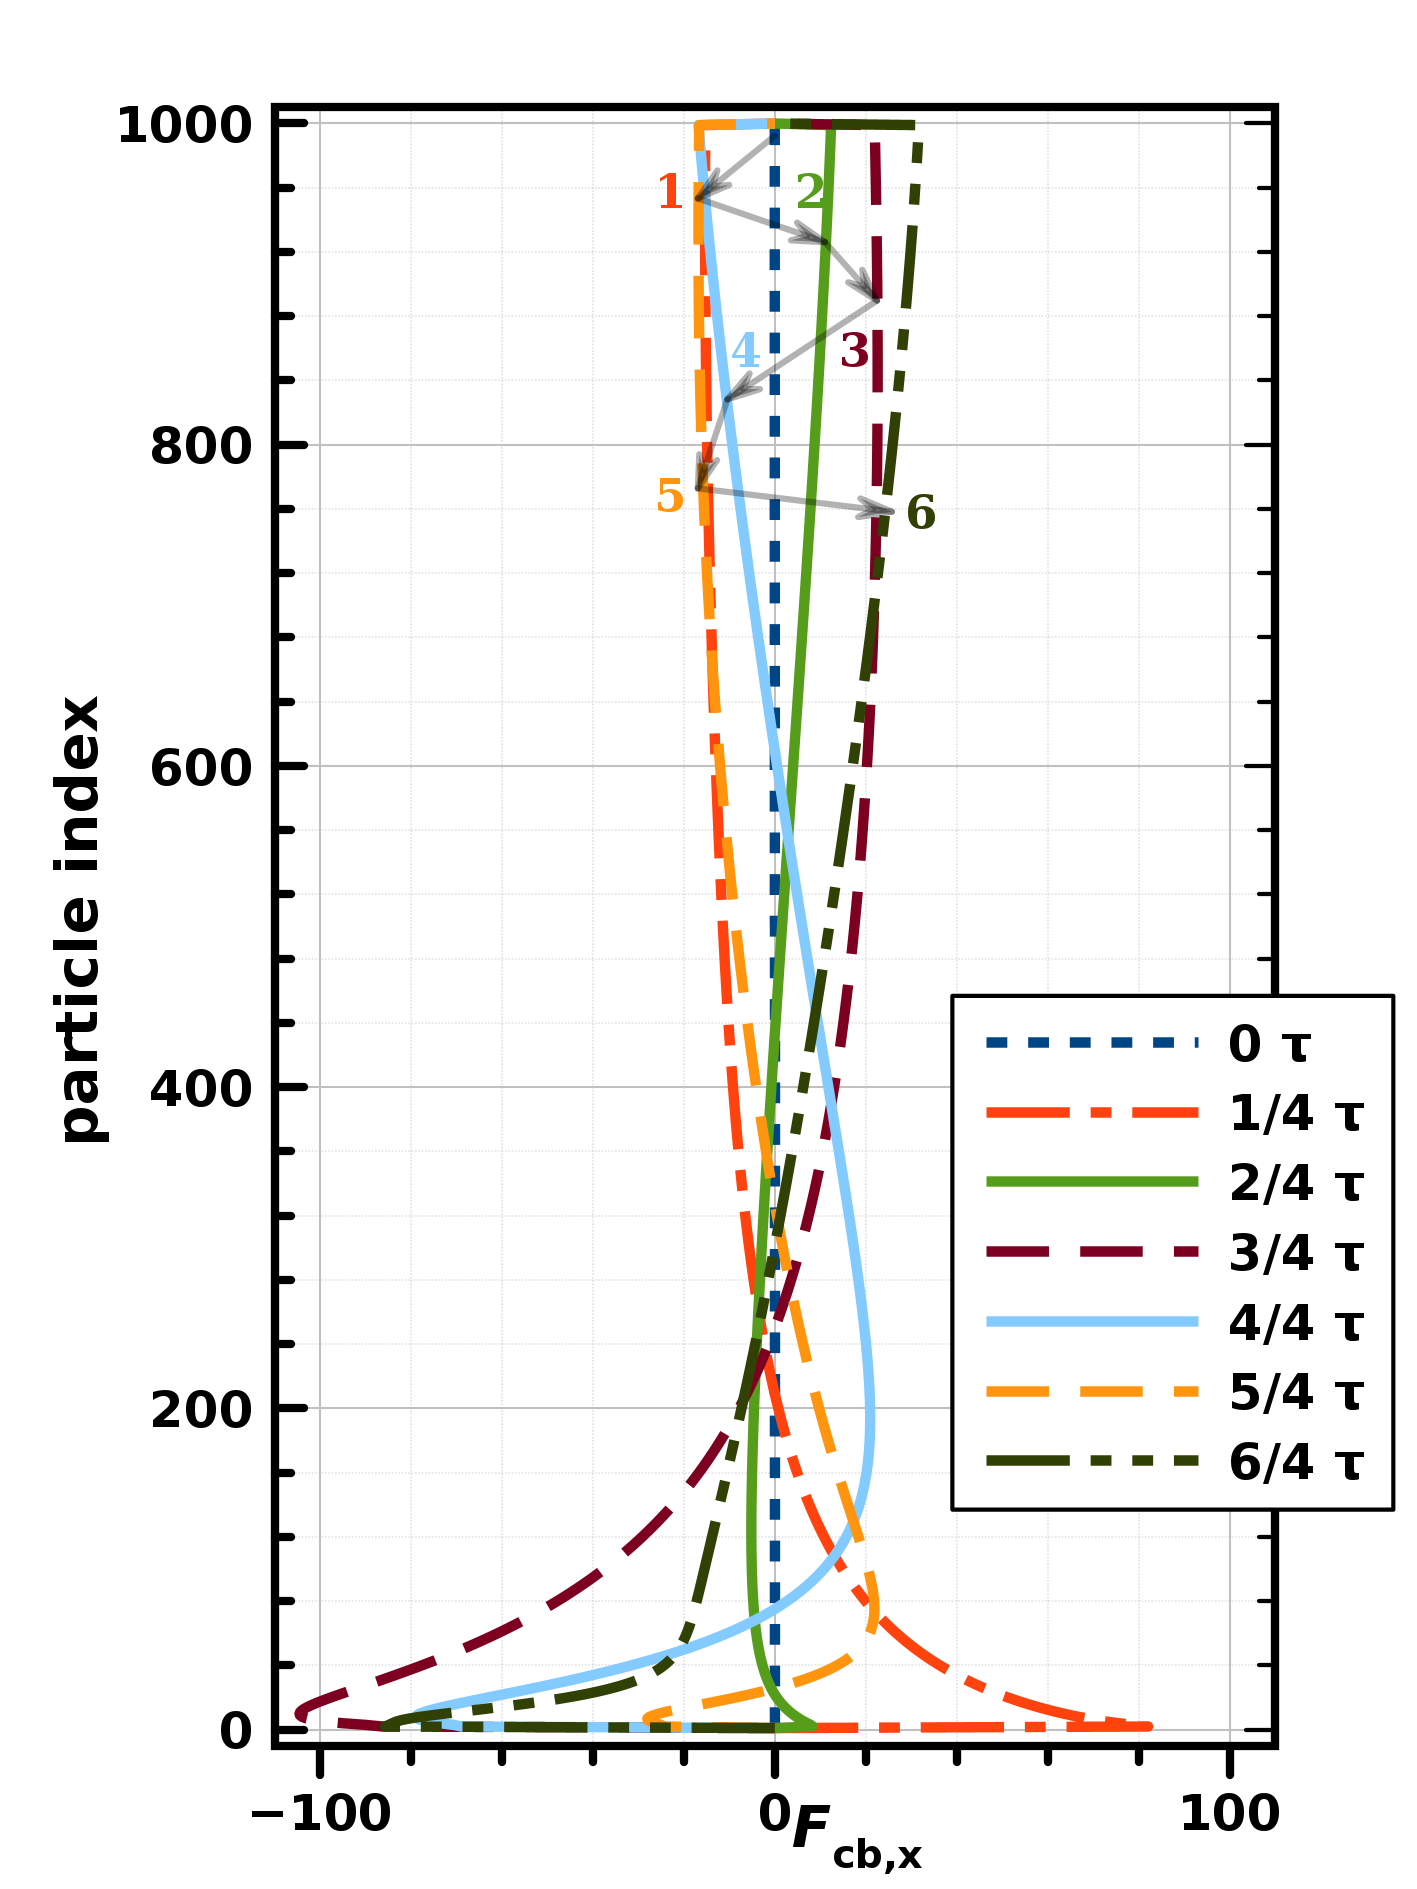
\includegraphics[width=1.75in]{figures/cXpvdf1000FC1}

\end{column} \begin{column}{.45\textwidth} % Right column and width
\centering 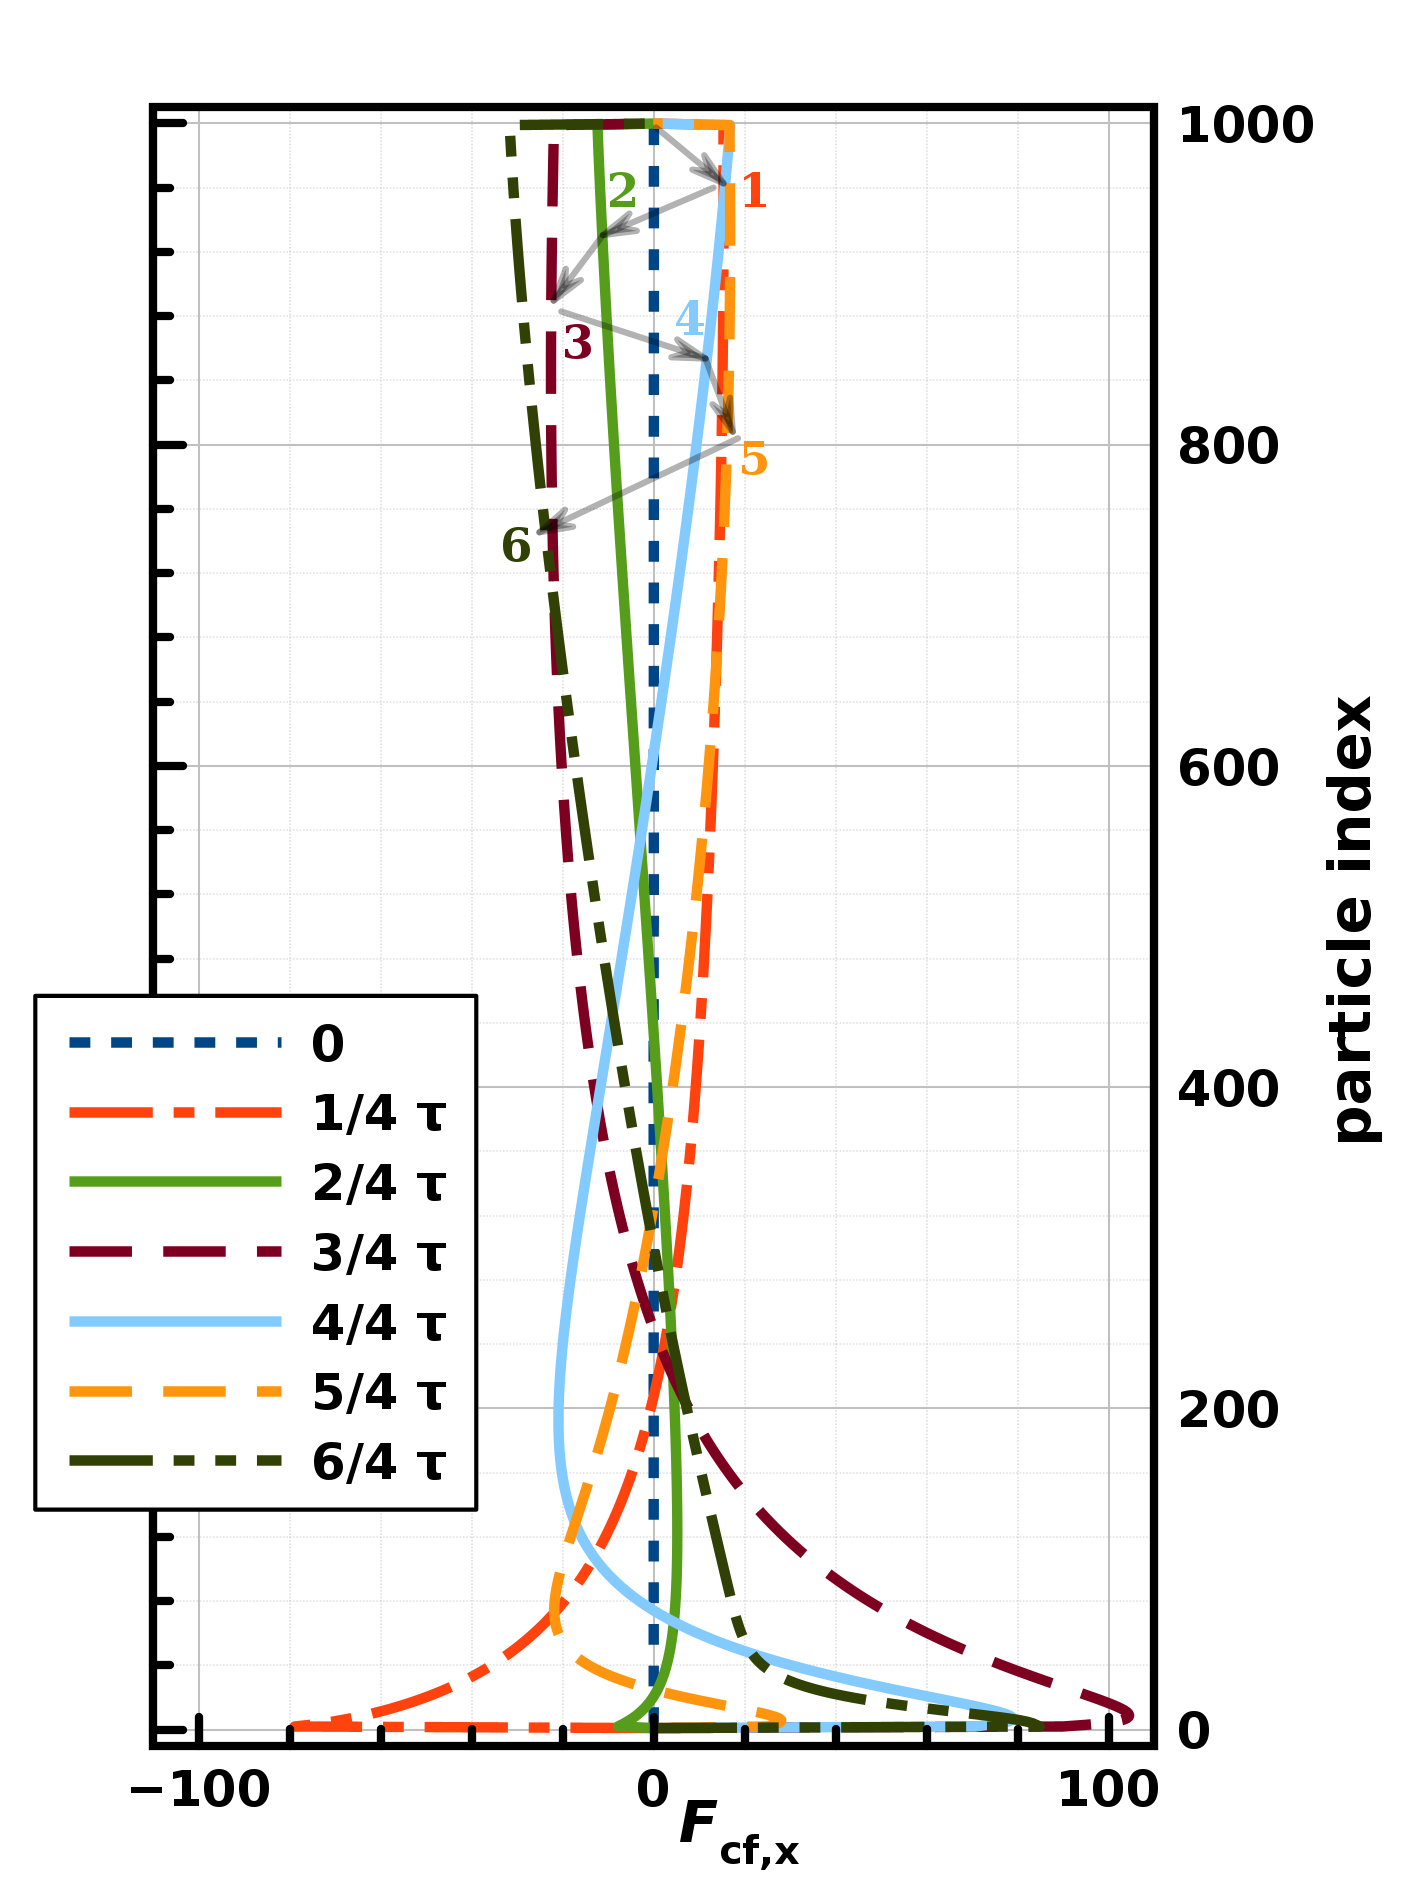
\includegraphics[width=1.75in]{figures/cXpvdf1000FC2}

\end{column} 
\end{columns}

\end{frame}
%
\begin{frame}[label={sec:org843a995}]{{[}Long Chain{]} Constraint Forces in $z-$ Direction}
\begin{itemize}
\item The periodicity and anti-symmetry become less apparent. 
\item Constraint force unit {[}nN{]} 
\end{itemize}
\begin{columns}[c]
% The "c" option specifies centered vertical alignment
% while the "t" option is used for top vertical alignment
\begin{column}{.45\textwidth} \centering 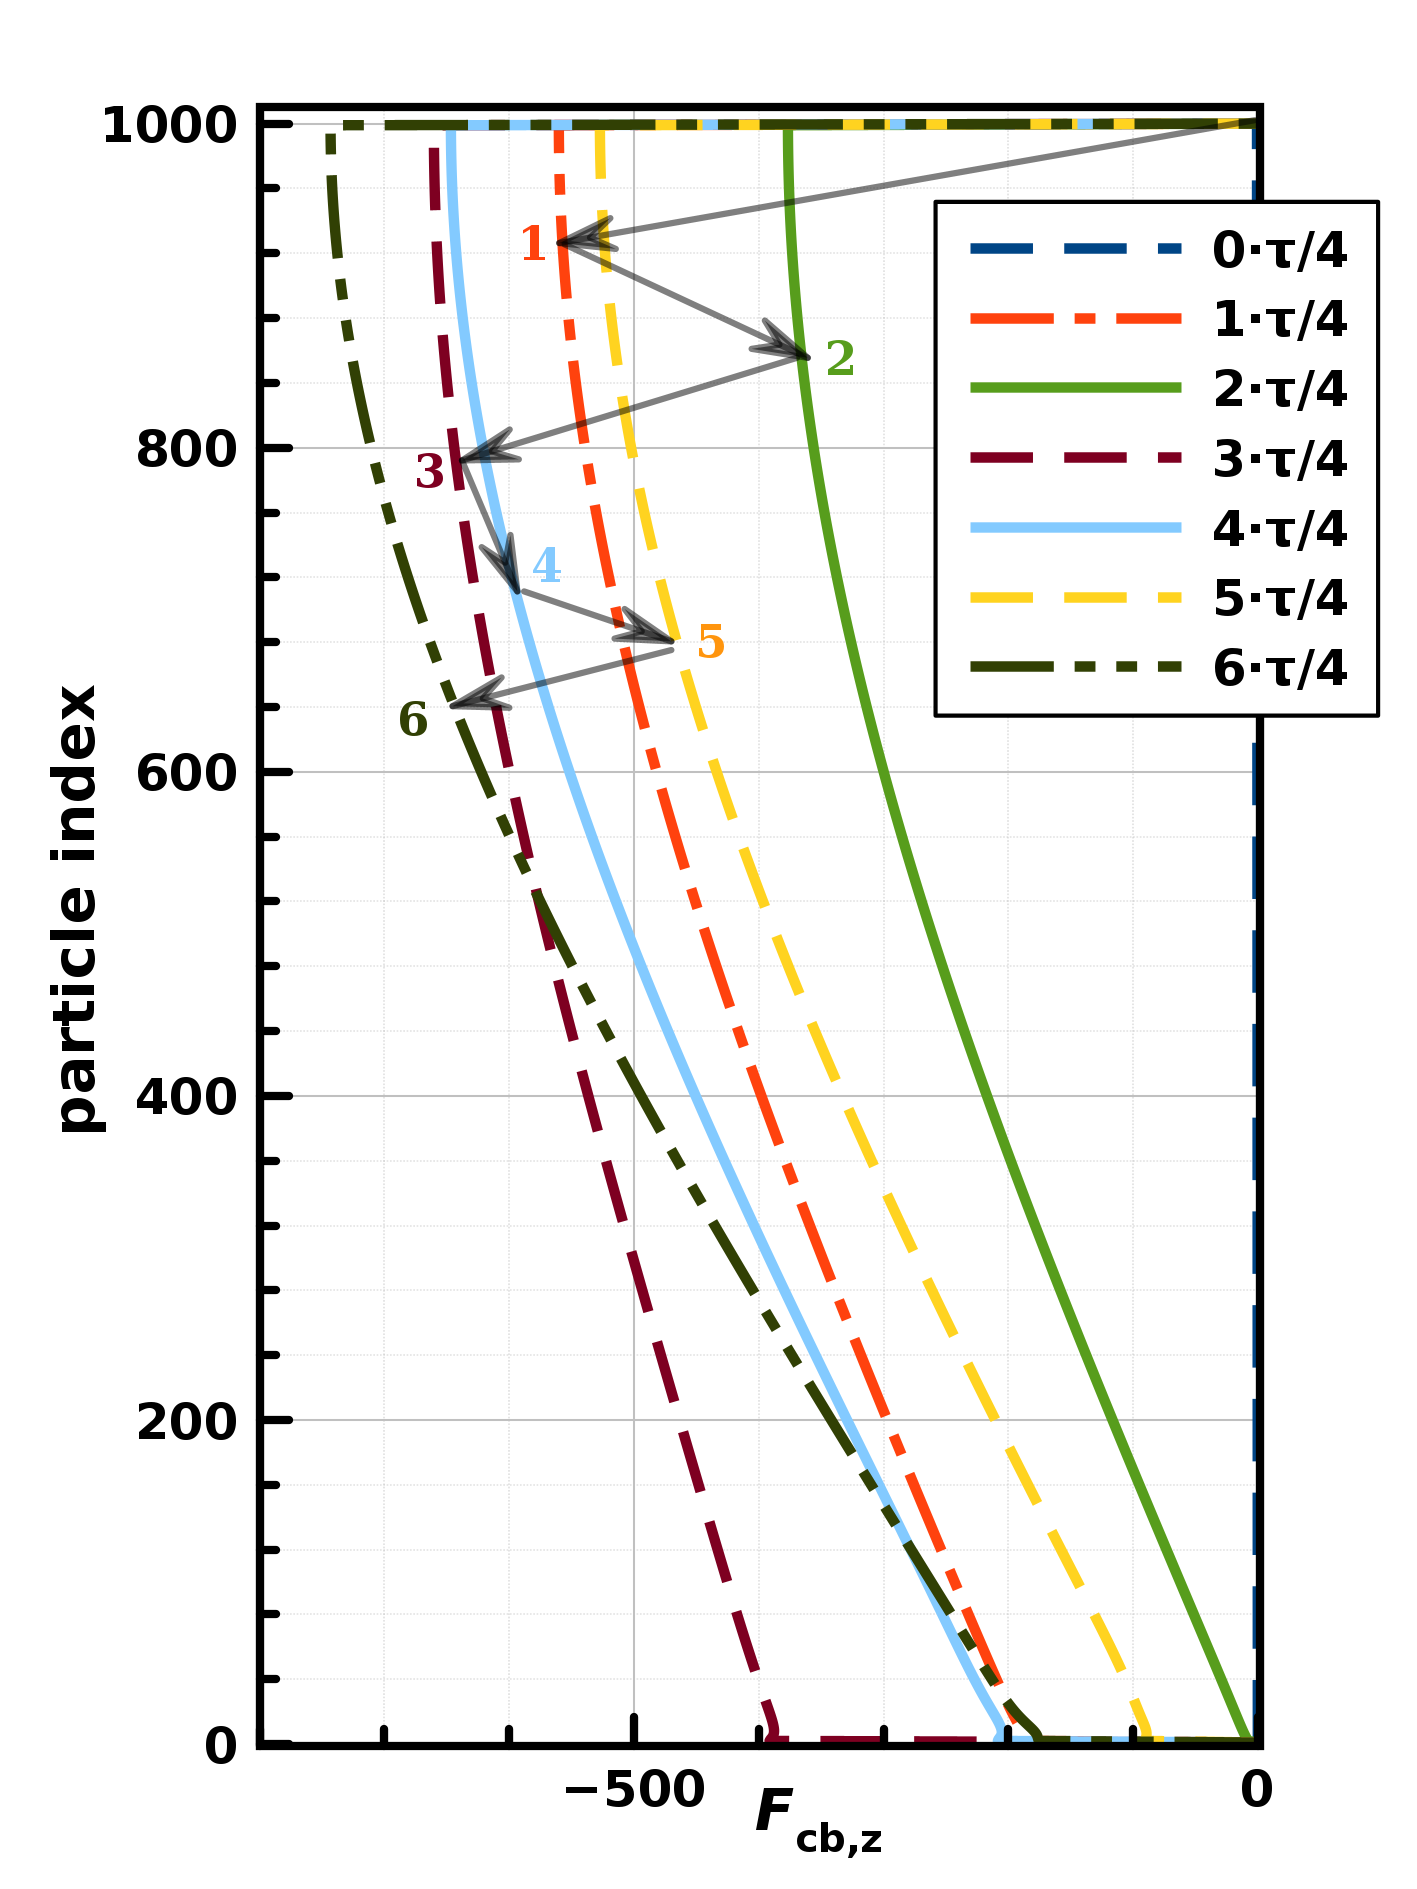
\includegraphics[width=1.75in]{figures/cZpvdf1000FC1}

\end{column} \begin{column}{.45\textwidth} % Right column and width
\centering 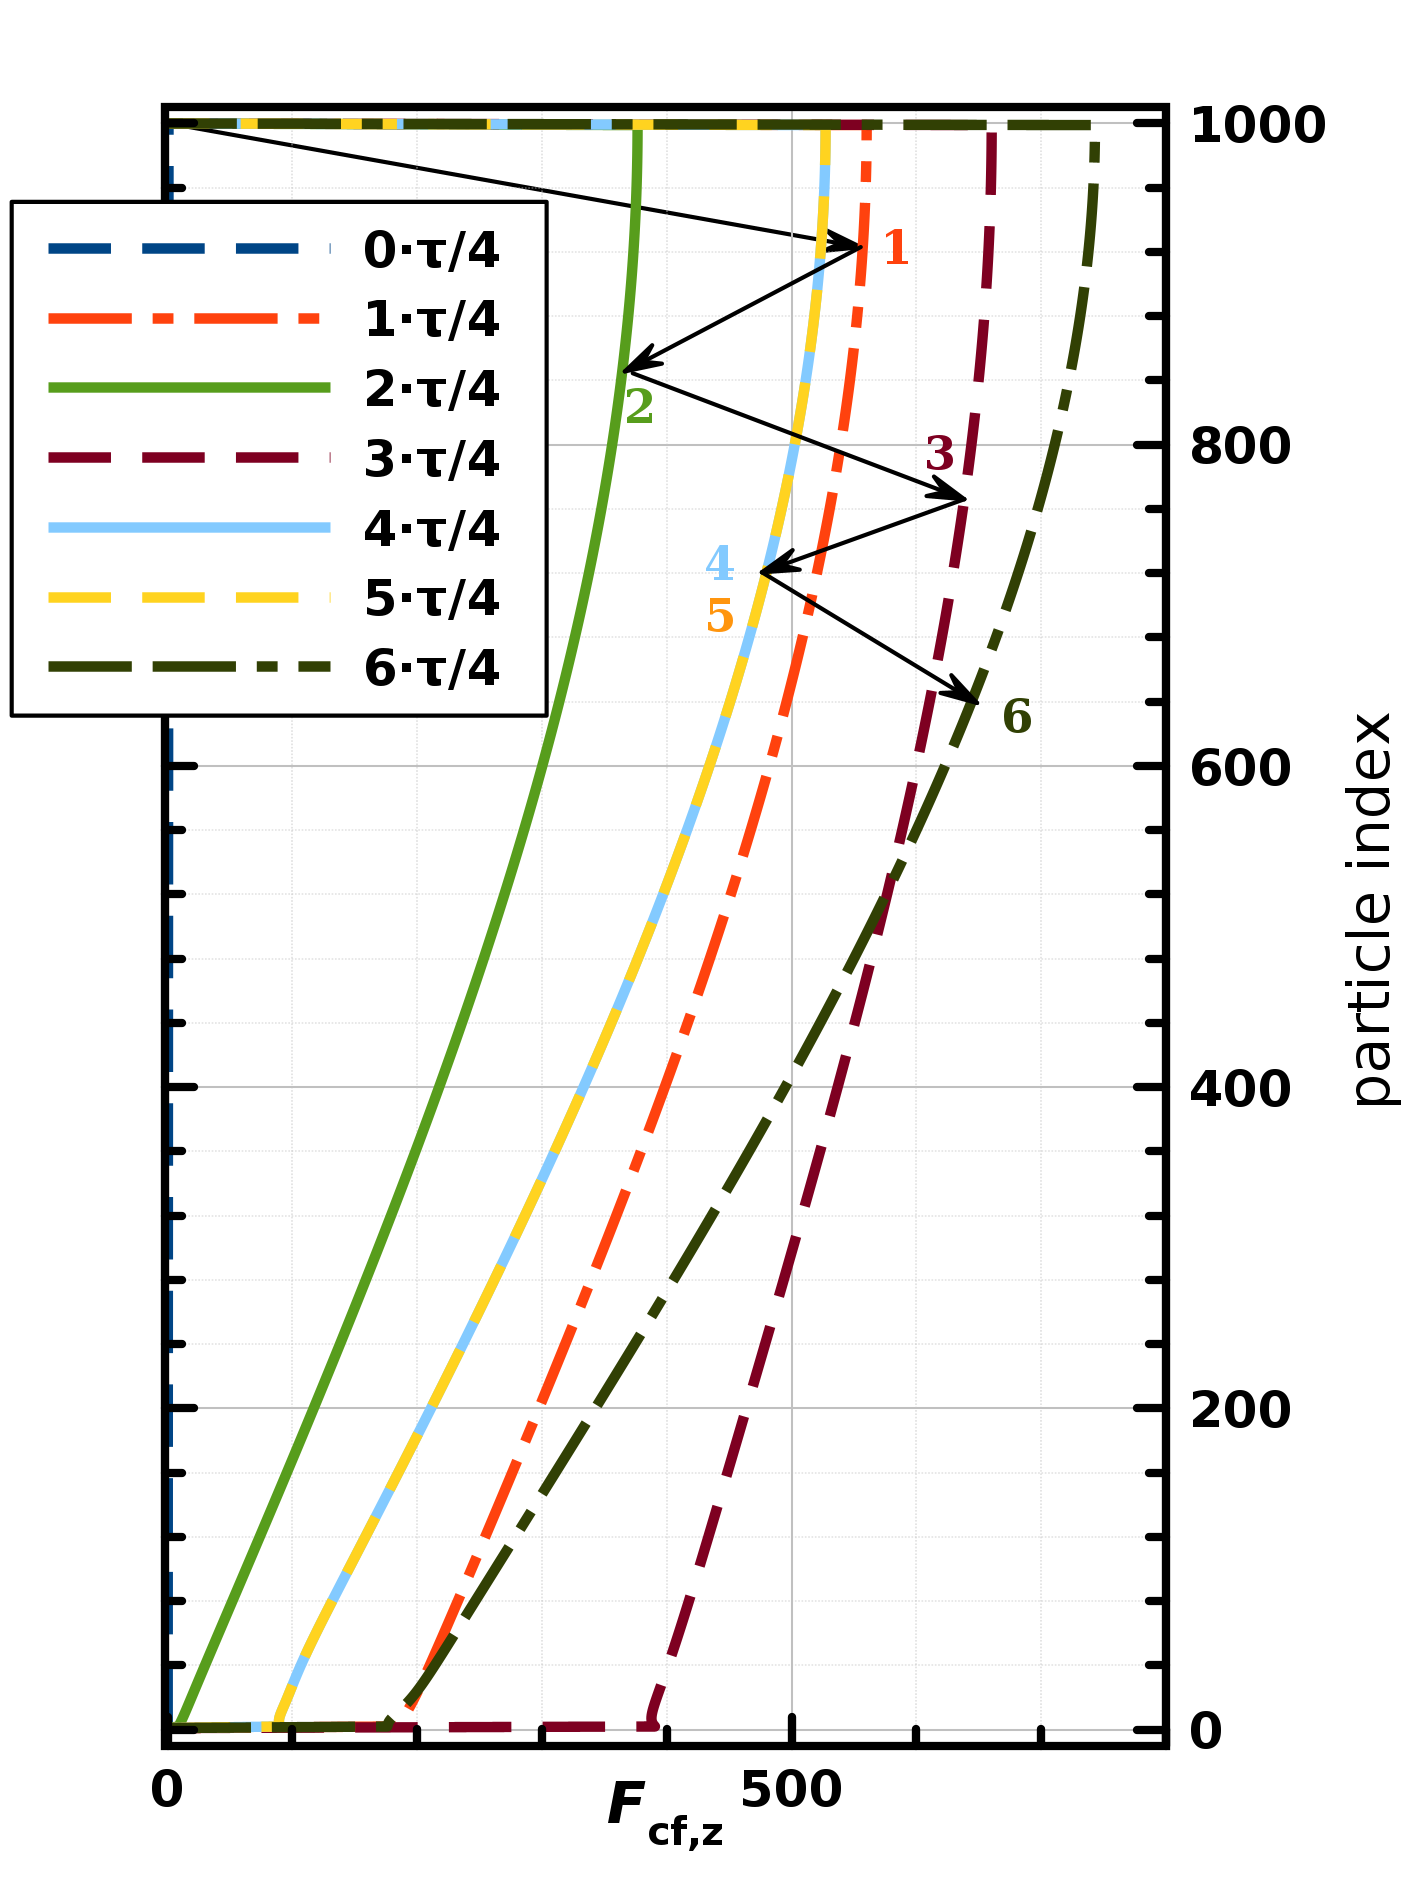
\includegraphics[width=1.75in]{figures/cZpvdf1000FC2}

\end{column} 
\end{columns}

\end{frame}
%
\begin{frame}[label={sec:orgf0ccd2c}]{{[}Long Chain{]} Total Force in $x-$ and $z-$ Direction}
\begin{itemize}
\item Unexpected similarity instead of periodicity in $F_{tot}$ {[}$\mu{\rm {N}}${]} 
\end{itemize}
\begin{columns}[c]
% The "c" option specifies centered vertical alignment
% while the "t" option is used for top vertical alignment
\begin{column}{.45\textwidth} \centering 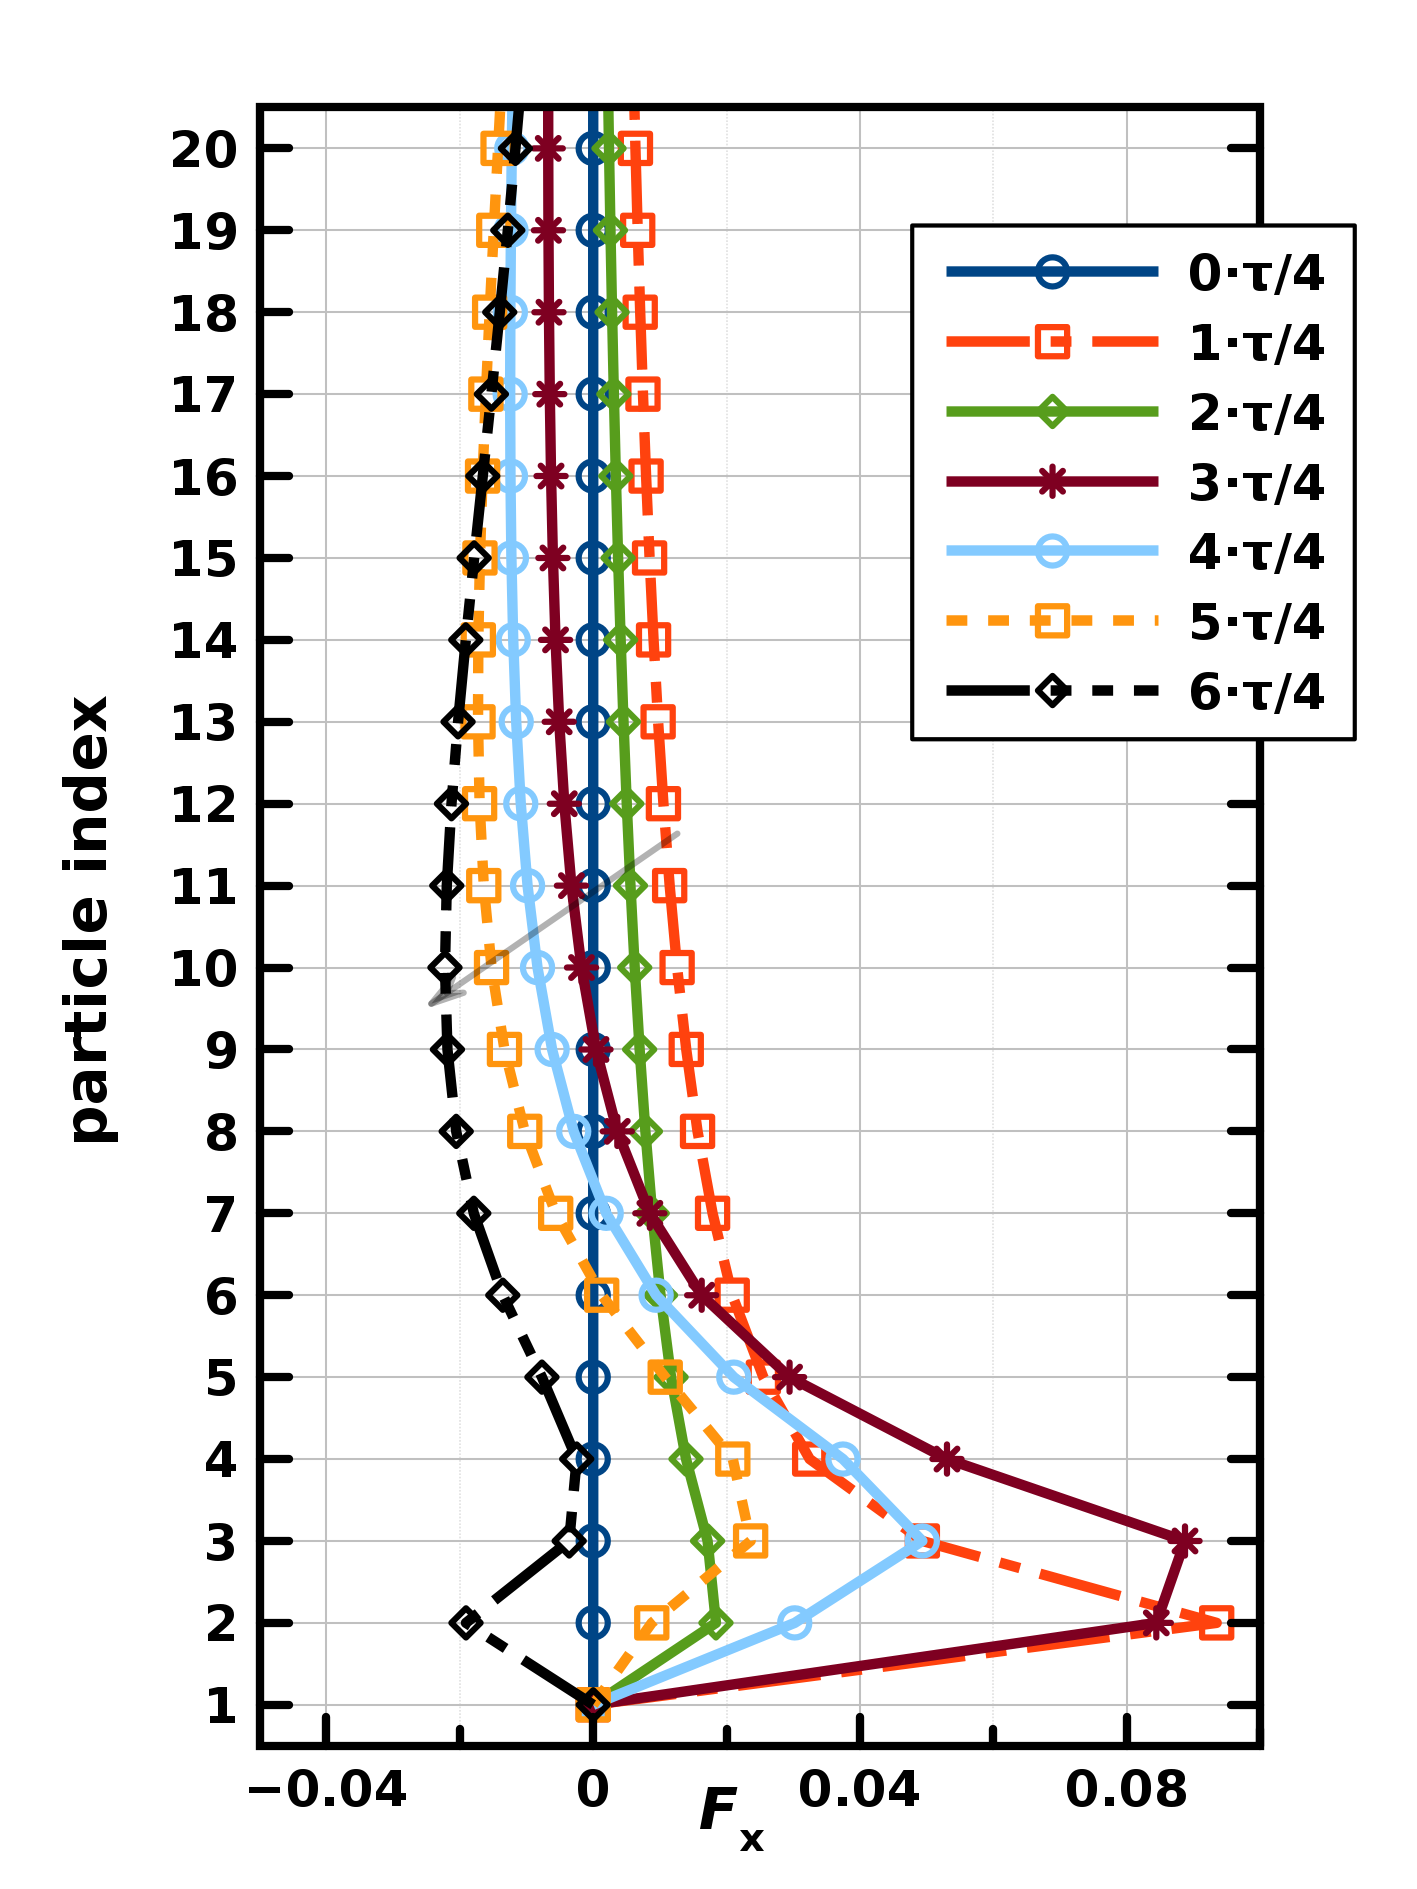
\includegraphics[width=1.75in]{figures/cXpvdf1000FTS}

\end{column} \begin{column}{.45\textwidth} % Right column and width
\centering 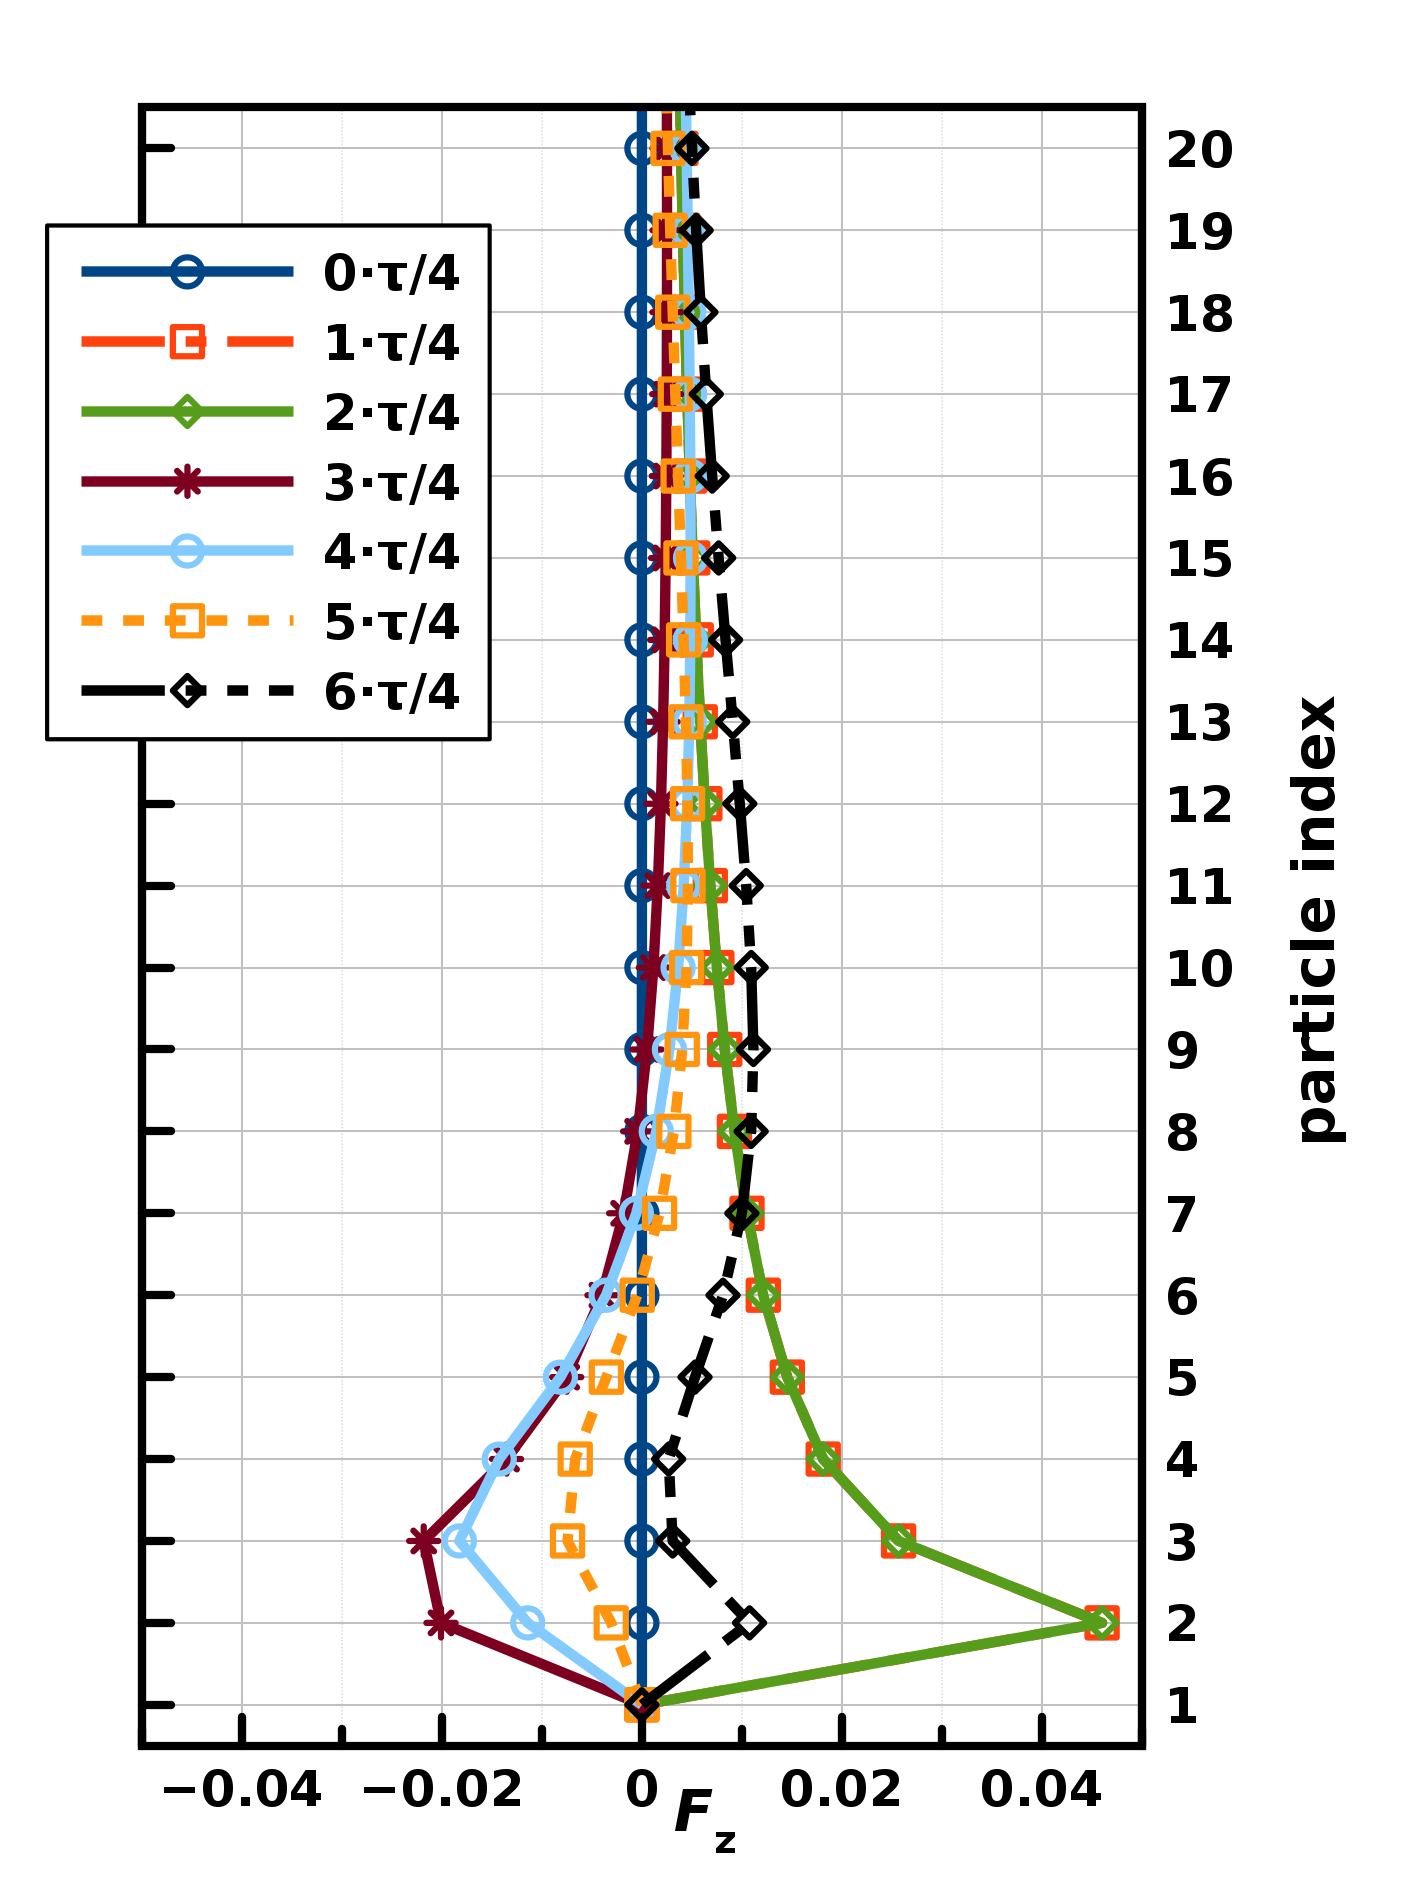
\includegraphics[width=1.75in]{figures/cZpvdf1000FTS}

\end{column} 
\end{columns}

\end{frame}

\section{Concluding Remarks}

\label{sec:org3c1e452} 

\subsection{Conclusions}

\label{sec:org106c3c1} 
\begin{frame}[label={sec:orgcfdb9fe}]{Summary}
\begin{enumerate}
\item A single hollow fiber is modeled as a sphere-connected chain using
the equivalent sphere. 
\item A short chain reciprocation is within intuitive expectation. 
\item A long chain's geometrical configuration is less predictable. Because 
\begin{enumerate}
\item the return of the full fiber (i.e., the middle zone) is always after
the returning of the rack. 
\item hollow fiber motion is energy-dissipative and entropy-increasing. 
\item periodicity is not fully conserved, generating random/chaotic displacements 
\item perhaps good for fouling reduction, but against the fiber durability. 
\end{enumerate}
\end{enumerate}
\end{frame}

\section{Acknowledgment}

\label{sec:org2de8b9b} 

\subsection{Thank You}

\label{sec:org4abef29} 
\begin{frame}[label={sec:org8a05f38}]{Acknowledgment}
\begin{block}{Kolon Industry, Inc.}
\begin{center}

\includegraphics[width=2in]{figures/kolon-logo} \label{org3dbc5a4} 
\par\end{center}
\vspace{-0.25cm}
 {\large{}\centering }\textbf{\large{}KO}{\large{}rea + Ny}\textbf{\large{}LON}{\large{}
= KOLON (from 1957) }{\large\par}
\end{block}
\end{frame}
%
\begin{block}{Korea Res. Inst. of Ships and Ocean Engineering (KRISO)}
\emph{For steady support and long-term collaborators \ldots} 
\begin{block}{}
\begin{center}

\includegraphics[width=1.75in]{figures/KRISO} \label{org8f512b1} 
\par\end{center}

\end{block}
\end{block}
%
\begin{frame}[label={sec:org80737df}]{Contact Information}
\centering \vspace{0.3cm}
 \textit{Hydrodynamic load exerted on a moving bundle of hollow fibers
using constraint dissipative hydrodynamics: Hydro-Rattle simulation}

\vspace{0.3cm}
 Albert S. Kim, Professor 

\vspace{0.3cm}
 Civil and Environmental Engineering

College of Engineering $|$ University of Hawai\textquoteleft i at
Mānoa 

(808) 956-3718 $|$ albertsk@hawaii.edu 

\vspace{0.3cm}
 \url{http://www.eng.hawaii.edu} $|$ \url{http://albertsk.org} 

\vspace{0.3cm}
 
\end{frame}
%
\begin{frame}[label={sec:org2f49c0e}]{Questions and Comments?}
\begin{center}

\includegraphics[width=4in]{figures/Question-mark} 
\par\end{center}
\end{frame}

\end{document}
